\documentclass[12pt]{dalthesis}
%\usepackage[utf8]{inputenc}
\usepackage{graphicx}
%\usepackage{tgtermes} 
\graphicspath{ {images/} }
\usepackage{mathtools}
\usepackage{amssymb}
\usepackage{amsfonts}
\usepackage{fancyvrb}
\usepackage{tikz}
\usepackage{tikz-qtree}
\usepackage{listings}
\usepackage{multicol}
\usepackage{amsthm}
\usepackage{amsmath }
\usepackage{xcolor}
\usepackage{framed}
\usepackage{color,soul}
\usepackage{tikz-cd}
\usetikzlibrary{matrix,arrows,decorations.pathmorphing, shadows, trees}
\usepackage{nomencl}
\usepackage{geometry}
\usepackage{setspace}
\usepackage{enumerate}
%%
%% Maple definitions (c) 2008 Alexander Shapiro
%%
\lstdefinelanguage{Maple}
{keywords={and,assuming,break,by,catch,description,do,done, elif,else,end,error,export,fi,finally,for,from,global,if, implies,in,intersect,local,minus,mod,module,next,not,od,%
option,options,or,proc,quit,read,return,save,stop,subset,then, to,try,union,use,uses,while,xor},
sensitive=true,
morecomment=[l]\#,
morestring=[b]",
morestring=[d]"
}[keywords,comments,strings]

\definecolor{mygreen}{RGB}{34,139,34}
\definecolor{mygray}{rgb}{0.5,0.5,0.5}
\definecolor{mymauve}{rgb}{0.58,0,0.82}

\lstset{ 
   xleftmargin=-25pt,
   xrightmargin=-25pt,
   framesep=0pt,
  backgroundcolor=\color{white},   % choose the background color; you must add \usepackage{color} or \usepackage{xcolor}; should come as last argument
  basicstyle=\small,        % the size of the fonts that are used for the code
  breakatwhitespace=true,         % sets if automatic breaks should only happen at whitespace
  breaklines=true,                 % sets automatic line breaking
%  captionpos=b,                    % sets the caption-position to bottom
  commentstyle=\color{mygreen},    % comment style
%  deletekeywords={...},            % if you want to delete keywords from the given language
%  escapeinside={\%*}{*)},          % if you want to add LaTeX within your code
%  extendedchars=true,              % lets you use non-ASCII characters; for 8-bits encodings only, does not work with UTF-8
%  firstnumber=5,                % start line enumeration with line 1000
  frame=single,	                   % adds a frame around the code
  keepspaces=false,                 % keeps spaces in text, useful for keeping indentation of code (possibly needs columns=flexible)
  keywordstyle=\bfseries\color{blue},       % keyword style
  language=Maple,                 % the language of the code
  morekeywords={*,...},            % if you want to add more keywords to the set
  numbers=left,                    % where to put the line-numbers; possible values are (none, left, right)
  numbersep=5pt,                   % how far the line-numbers are from the code
  numberstyle=\color{black}, % the style that is used for the line-numbers
  rulecolor=\color{black},         % if not set, the frame-color may be changed on line-breaks within not-black text (e.g. comments (green here))
  showspaces=false,                % show spaces everywhere adding particular underscores; it overrides 'showstringspaces'
  showstringspaces=false,          % underline spaces within strings only
  showtabs=false,                  % show tabs within strings adding particular underscores
  stepnumber=1,                    % the step between two line-numbers. If it's 1, each line will be numbered
  stringstyle=\color{mymauve},     % string literal style
  tabsize=2,	                   % sets default tabsize to 2 spaces
  title=\lstname                   % show the filename of files included with \lstinputlisting; also try caption instead of title
}



\theoremstyle{plain}
\newtheorem{theorem}{Theorem}
\newtheorem{corollary}{Corollary}
\newtheorem*{corollary*}{Corollary}
\newtheorem{proposition}{Proposition}
\newtheorem*{proposition*}{Proposition}
\newtheorem{definition-proposition}{Definition-Proposition}
\newtheorem{lemma}{Lemma}
\newtheorem*{lemma*}{Lemma}
\newtheorem{conjecture}{Conjecture}
\newtheorem*{conjecture*}{Conjecture}

\theoremstyle{definition}
\newtheorem{example}{Example}
\newtheorem{construction}{Construction}
\newtheorem{notation}{Notation}
\newtheorem*{notation*}{Notation}
\newtheorem{definition}{Definition}
\newtheorem*{definition*}{Definition}
\newtheorem{observation}{Observation}
\newtheorem*{observation*}{Observation}
\newtheorem{question}{Question}
\newtheorem*{question*}{Question}

\begin{document}

\title{title}
\author{Anne Johnson}

\mcs

\degree{Master of Science}
\degreeinitial{M.Sc.}
\faculty{Science}
\dept{Faculty of Mathematics}


% Month and Year of Defence
\defencemonth{August}\defenceyear{2019}

\dedicate{Optionally, the thesis can be dedicated to someone, and the
  student can enter the dedication content here.}

%\nolistoftables
%\nolistoffigures

%\frontmatter


%\begin{abstract}
%	something about math
%\end{abstract}

%\begin{acknowledgements}
%  remember to thank people
%\end{acknowledgements}

\mainmatter

%\chapter{Introduction}
%\begin{itemize}
\item Provide motivation and context to various definitions of capacity and p-orderings
\item Show the following examples of generalizations : product spaces, finite/algebraic extensions of $\mathbb{Z}_p $, projective space
\end{itemize}
\chapter{Capacity and Ultrametric spaces}
\section*{Ultrametric basics}


\begin{definition*}
	 Let $(M, \rho)$ be a metric space. If $\rho$ satistifies the ultrametric inequality
	\[\rho(x,z) \leq max{(\rho(x,y), \rho(y,z))}, \forall x,y,z \in M\] 
	then (M, $\rho$) is an \textbf{ultrametric space}.
\end{definition*}

\begin{definition*}
	 Let $(V, N)$ be a normed vector space. Then $N$ satisfies the \textbf{strong trianlge inequality} if
	\[N(x + y) \leq max(N(x), N(y)), \forall x,y \in V \]
\end{definition*}

\begin{proposition*}
	Let $(V,N)$ be a normed vector space and suppose $N$ satisfies the strong triangle inequality. Then the metric space, $(V,\rho_N)$, where $\rho_N$ is the metric induced by $N$, is an ultrametric space.
\end{proposition*}

\begin{proposition*}
	\cite{ar} All triangles in an ultrametric space $(M,\rho)$ are either equilateral or isocoles, with at most one short side. 
\end{proposition*}


\begin{proposition*}
\cite{ar} If $S$ is a compact subset of an ultrametric space and $\Gamma_S$ is the set of all distances occurring between points of $S$, then $\Gamma_S$ is a discrete subset of $\mathbb{R}$. In particular if $\mid \Gamma_S\mid = \infty$, then the elements of $\Gamma_S$ can be indexed by $\mathbb{N}$.
\end{proposition*}

\noindent Let $(M, \rho)$ be a compact ultrametric space and let \[B_r(a)=\{x \in M \mid \rho(x,a) < r\}\] denote the open ball of radius $r$, centred at $a$ for some $r \in \mathbb{R}_{\geq 0}$ and $a \in (M,\rho)$. Likewise let \[\overline{ B_r(a)}=\{x \in M \mid \rho(x,a) \leq r\}\]  denote the closed ball of radius $r$, centred at $a$ for some $r \in \mathbb{R}_{\geq 0}$ and $a \in (M,\rho)$.

\begin{proposition*}
	Let $B_r(a)$ be a ball in an ultrametric space $(M,\rho)$. Then the diameter of $B$, $d=diam(B)=\sup_{x,y \in B}{\rho(x,y)}$, is less than or equal to the radius of $B$.    
\end{proposition*}

\begin{proposition*}
	If $(M, \rho)$ is an ultrametric space and $B_{r_1}(x_0)$ and $B_{r_2}(y_0)$ are balls in $(M, \rho)$, then either $B_{r_1}(x_0) \cap B_{r_2}(y_0) = \emptyset$, $B_{r_1}(x_0) \subseteq B_{r_2}(y_0)$, or $B_{r_2}(x_0) \subseteq B_{r_1}(x_0)$. That is, in an ultrametric space, all balls are either comparable or disjoint.
\end{proposition*}

\begin{proposition*}
\cite{ar} The distance between any two balls in an ultrametric is constant. That is, if $B_{r_1}(x_0)$ and $B_{r_2}(y_0)$ are two balls in an ultrametric space $(M,\rho)$, then $\rho(x,y)=c$ for some $c \in \mathbb{R}$ and $\forall x \in B_{r_1}(x_0)$ and $\forall y \in B_{r_2}(y_0)$
\end{proposition*}

\begin{proposition*}
\cite{ar} Every point of a ball in an ultrametric is at its centre. That is, if $B_r(x_0)$ is a ball in an ultrametric space $(M,\rho)$, then $B_r(x)=B_r(x_0)$,  $\forall x \in B_r(x_0)$
\end{proposition*}




\chapter{$\rho$-orderings and the structure of $S$}

In the previous section, we defined valuative capacity for a compact subset $S$ of an ultrametric space $(M, \rho)$. We also got a glimpse into the way the valuative capacity of $S$ interacts with its other properties, such as the set of distances occurring in $S$ and the lattice of closed balls in $S$ (or equivalently, if $S$ has enough structure, a lattice of subgroups).\\

In this section, we offer a more detailed study of the interaction between the valuative capacity of $S$ and the lattice of closed balls in $S$. In particular, we  show how, if $S$ is compact and discretely-valued, the lattice of closed balls can be used to compute the first $n$ terms of a $\rho-$ordering of $S$ (for any $n < \infty$). In the following chapter we show how, in some cases, this extends to being able to derive a formula for the valuative capacity of $S$.\\

Similar results have been found for the special case of ultrametric fields in \cite{cef}. We extend these results by moving to a more general setting, showing that much can be said about capacity in $S$ without appealing to any underlying algebraic structure. Significant portions of the theory developed in this chapter was guided by an empirical investigation into the capacity of product spaces, which we describe in the next chapter. The code that performed these calculations is included in the appendix.\\

We assume throughout this section that $S$ is a compact, discretely-valued subset of an ultrametric space $(M, \rho)$.\\

\subsection*{Subspaces of $S$}
In the section we explore the subspaces of $S$ formed by considering closed balls of some fixed radius.  Recall from the previous section that if $S$ is compact and discretely-valued, then the set of distances occurring in $S$ is a discrete, bounded subset of $\mathbb{R}$ and so we may represent the set of distances by a sequence in decreasing order. As before, let the decreasing sequence of distances in $S$ be given by  $\Gamma_S =\{\gamma_0=\text{diam}(S), \gamma_1,\ldots,\gamma_\infty=0\}$.\\

 Now fix some $k \in \mathbb{N}$, and consider for a moment the set of closed balls of radius $\gamma_k$ in $S$. We could denote these alternatively by $B^M(x, \gamma_k) \cap S$ or by  $B^S(x, \gamma_k)$, but when there is no risk of confusion, we will denote them simply by $B(x, \gamma_k)$. Clearly, the set  $\{B(x, \gamma_k); x \in S\}$ forms a cover of $S$. Although we have build the cover using closed balls, since we are in an ultrametric space, this gives an open cover of $S$ (in fact, each element in the cover is not only an open set, but also an open ball for some radius slightly bigger than $\gamma_k$). Then since $S$ is compact, we must have some $x_1,\ldots, x_n$  such that $S= \cup_{i=1}^n B(x_i, \gamma_k)$. In fact,  since $\rho$ is an ultrametric, we can pick the $x_i$'s so that $\cup_{i=1}^n B(x_i, \gamma_k)$ will be a disjoint union and therefore a finite partition of $S$. Note that both $n$ and the $x_i$'s depend on our fixed $k$, but that $n$ is independent of the $x_i$'s, since any choice of centres is equivalent. We rephrase this with following definition and lemma:\\

\begin{definition}
For $S$ and $\Gamma_S$ as above, and $k \in \mathbb{N}$, fixed,  define $\sim_k$ to  be the relation on $S$ given by \[x \sim_k y\text{ if and only if  }\rho(x,y) \leq \gamma_k\] i.e.,  $x \sim_k y$ if and only if $B_{\gamma_k}(x) = B_{\gamma_k}(y)$.
\end{definition}

The fact $\sim_k$ is an equivalence relation on $S$ is equivalent to the observation that every point in a ultrametric ball is at its centre:\\

\begin{lemma}
Let  $S$ and $\Gamma_S$ be as above, then $\sim_k$ is an equivalence relation on $S$.
\end{lemma}

\begin{proof}
$\sim_k$ is clearly reflexive and symmetric, since $\rho$ is a metric. Transitivity results from the ultrametric property of $\rho$: if $x \sim_k y$ and $y \sim_k z$, then $$\rho(x, z) \leq \max(\rho(x,y), \rho(z,y)) \leq \gamma_k$$ so $x \sim_k z$. 
\end{proof}

 We denote the set of equivalence classes of $S/\sim_k$ by $S_{\gamma_k}$. We have defined  $S_{\gamma_k}$ to be the set of equivalence classes in $S$ under the relation $\sim_k$, which is equivalent to letting $S_{\gamma_k}$ be the set of closed balls of fixed radius $\gamma_k$ in  $S$. We now offer a third perspective on the elements on $S_{\gamma_k}$, which is due to \cite{na},\\

\begin{lemma}
For each $k$, the elements of $S_{\gamma_k}$, that is, the closed balls of radius $\gamma_k$, themselves form an ultrametric space, where the metric is given by:
\[ \rho_k(B(x, \gamma_k),B(y, \gamma_k)) = 
\begin{cases}
\rho(x,y), & \text{if } \rho(x,y) > \gamma_k \\
0, & \text{if }   \rho(x,y) \leq \gamma_k \text{, i.e., } B(x, \gamma_k)=B(y, \gamma_k)
\end{cases}
\]
\end{lemma}

\begin{proof}
$\rho_k$ is reflexive, symmetric and transitive since $\rho$ is. Likewise, $\rho_k$ satisfies the ultrametric property, since $\rho$ does: let $B(x, \gamma_k),B(y, \gamma_k)$ and $B(z, \gamma_k)$ be any three elements of $S_{\gamma_k}$ and suppose $\rho_k(B(x, \gamma_k),B(y, \gamma_k)) > 0 $. Then,
\begin{align*}
\gamma_k < \rho_k(B(x, \gamma_k),B(y, \gamma_k)) && \\
= \rho(x,y) \leq \max(\rho(x,z), \rho(y,z)) && \\
= \max(\rho_k(B(x, \gamma_k), B(z, \gamma_k)), \rho_k(B(y, \gamma_k),B(z,\gamma_k)))
\end{align*}
since $ \gamma_k < \max(\rho(x,z), \rho(y,z))$ implies that at least one of $\rho_k(B(x, \gamma_k), B(z, \gamma_k))$ or $\rho_k(B(y, \gamma_k),B(z,\gamma_k))$ is greater than $0$.
\end{proof}

So now the elements of $S_{\gamma_k}$ may be viewed as either equivalence classes, closed balls of fixed radius, or points in a new metric space. We  make a final definition and introduce some notation before moving on.\\

\begin{definition}
Let $S$ and $\Gamma_S$ be as above. Define $\beta(i)_{i \geq 0}$ to be the sequence given by $\beta(i) = \lvert  S_{\gamma_i}\rvert$, which is an invariant of $S$ and which counts the number of connected components of $S_{\gamma_i}$ (that is, the points of $S_{\gamma_i}$), when viewed as a metric space. When necessary, we use $\beta^S(i)$ to denote the $\beta$ sequence for a given, compact  ultrametric space $S$. Adapting the terminology in \cite{fp}, we call $\beta^S(i)$ the \textbf{structure sequence} of $S$.
\end{definition}

\begin{notation}
Let $S_{\gamma_k}$ be as above. We denote the elements of $S_{\gamma_k}$ by $B^k_1, \ldots, B^k_{\beta(k)}$ or by $B^{S,k}_1, \ldots, B^{S,k}_{\beta(k)}$, when necessary.
\end{notation}


We return to the sequence $\beta(i)$ at the end of this section. For now, we show how a $\rho-$ordering of $S$ can be built recursively from the spaces $S_{\gamma_k}$. This begins by noting that the spaces themselves can be built recursively:\\

\begin{observation}
Let $S$, $\Gamma_S$, and $S_{\gamma_k}$ be as above. Then $S_{\gamma_k+1}$ can be constructed by partitioning each of the closed balls in $S_{\gamma_k}$ into closed balls of radius $\gamma_{k+1}$ and taking their union:  Let $B(x_i, \gamma_k)$  be an element of $S_{\gamma_k}$, denoted by  $B^k_i$. Then, there exists $x_{i,1},\ldots, x_{i,l_{i}} \in B^k_i$ such that,

\[B^k_i=  \bigcup_{j=1}^{l_i} B(x_{i,j}, \gamma_{k+1})\] and  \[B(x_{i,j}, \gamma_{k+1}) \cap B(x_{i,j'}, \gamma_{k+1}) = \emptyset \text{, }\forall j,j' \in 1:l_i\]
and so

\[S_{\gamma_{k+1}} =  \bigcup_{i=1}^{\beta(k)}   \cup_{j=1}^{l_i} B(x_{i,j}, \gamma_{k+1}) = \bigcup^{\beta(k+1)}_{j=1}B^{k+1}_{j}\] 


where $\cup_{j=1}^{l_i} B(x_{i,j},\gamma_{k})=B(x_i, \gamma_{k+1}) = B^k_i$, $\forall i$.
\end{observation}

Since $S$ is compact, hence bounded, if we represent this process schematically we obtain a tree, where the root node is $B^0_1=B(x,\gamma_0)$, for any choice of $x \in S$, and the children of any given $B^m_n$ are such that they form a partition of their join.  Since we will often refer to this schematic representation, we define it below.\\

\begin{definition}
If $S$ is a compact subset of an ultrametric space, then $T_s$ is the tree whose vertices are $B^k_i$, that is the elements of $S_{\gamma_k}$, and whose edgeset, $E$, is given by $ (B^i_k, B^j_l) \in E$ if and only if $ j = i+1$ and $B^j_l \subseteq B^i_k$ for some choice of representatives $B(x_k,\gamma_i)$ and $B(x_l, \gamma_j)$, as shown below:\\

\tikzset{font=\small,
level distance=1.75cm,
}

\begin{center}
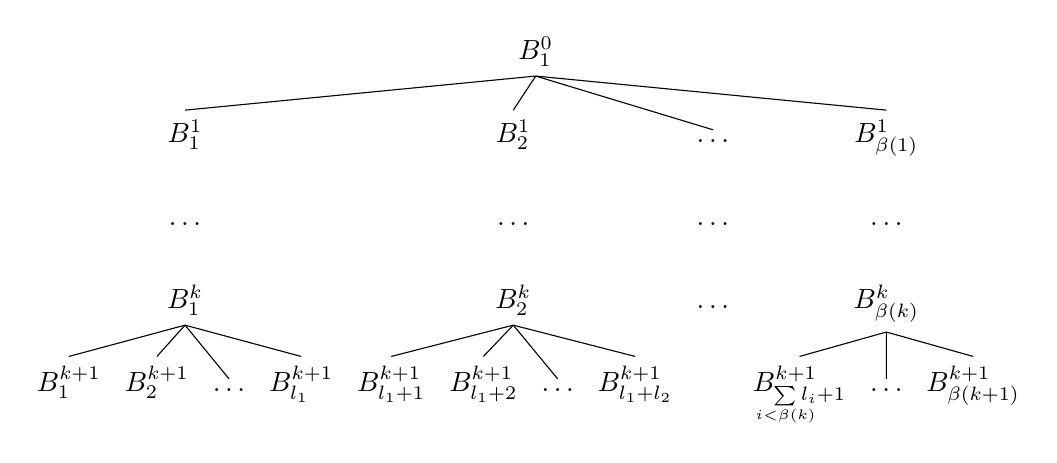
\begin{tikzpicture}
\Tree [. $B^0_1$ [. $B^1_1$ \edge [draw=none]; [. $\ldots$ \edge [draw=none]; [. $B^k_1$ [. $B^{k+1}_1$ ] [. $B^{k+1}_2$ ]  [. $\ldots$ ] [. $B^{k+1}_{l_1}$ ] ] ] ] 
		        [. $B^1_2$ \edge [draw=none]; [. $\ldots$ \edge [draw=none]; [. $B^k_2$ [. $B^{k+1}_{l_1 + 1}$ ] [. $B^{k+1}_{l_1 + 2}$ ] [. $\ldots$ ] [. $B^{k+1}_{l_1 + l_2}$ ] ] ] ] 
		        [. $\ldots$  \edge [draw=none]; [. $\ldots$ \edge [draw=none]; [. $\ldots$ ] ] ]
	                   [.$B^1_{\beta(1)}$ \edge [draw=none]; [. $\ldots$ \edge [draw=none]; [.$B^k_{\beta(k)}$ [. $B^{k+1}_{\sum\limits_{\mathclap{i < \beta(k)}}  l_i + 1 }$ ] [. $\ldots$ ] [. $B^{k+1}_{\beta(k+1)}$ ] ] ] ] ]
\end{tikzpicture}
\end{center}
\end{definition}

Before going on, first note that we have drawn $T_S$ such that leftmost child of some $B^k_i$ is $B^{k+1}_j$ where $j$ is minimal among the children of $B^k_i$, and then continued in increasing order. In general, if we draw $T_S$ so that the children of a given vertex are depicted in increasing order according to their index, then  each choice of indexing for the elements of $S_{\gamma_k}$ produces a different graphical representation of $T_S$. The structures produced by different choices of indices are clearly isomorphic as trees, and as we will see by the end of the section, each choice of indexing will be valid for our purposes as well.\\

Of central importance to us is the distance between two vertices in $T_s$. Since each vertex represents an element of $S_{\gamma_k}$, that is a closed ball in an ultrametric space, it is well-defined to let the distance between vertices be equal to the distance between a choice of centres for those balls. Note that if the distance between $B^k_i$ and $B^l_j$ is taken to be $\rho(x_i,x_j)$, for some choice of $x_i \in B^k_i$ and $x_j \in B^l_j$, say $\rho(x_i,x_j)=\gamma_n$, then the join of  $B^k_i$ and $B^l_j$ is some $B^n_x$.\\

\begin{lemma}
If $B^k_i$ and $B^l_j$ are two vertices in $T_S$, then $\rho(x_i,x_j)$, for any choice of  $x_i \in B^k_i$ and $x_j \in B^l_j$, is equal to the diameter of the join of  $B^k_i$ and $B^l_j$. 
\end{lemma}

\begin{proof}
Let $B^k_i$ and $B^l_j$ be two (distinct) vertices in $T_S$ and let $B^n_x$ be their join. The diameter of $B^n_x$ is $\gamma_n$ since $B^n_x=B(x_0, \gamma_n)$ for some $x_0$. Since $\rho$ is an ultrametric the distance between any  $x_i \in B^k_i$ and $x_j \in B^l_j$ is constant, and must be equal to the diameter of the smallest ball containing both of them, that is $\gamma_n$.
\end{proof}

In particular, we have that for any $k$ and any $i < \beta(k)$, the distances between the children of $B^k_i$ will be $\gamma_k$ and for any $i \neq j$ the distance between the children of $B^k_i$ and $B^k_j$ will be equal to the distance between  $B^k_i$ and $B^k_j$ (which will be some $\gamma_{m}, m <k$).\\

\section*{Recusive $\rho$-orderings}
In this section, we show how the recursive partioning of $S$ into the spaces $S_{\gamma_k}$ gives rise to a $\rho-$ordering of $S$. We first note that without loss of generality, for any $k \in \mathbb{N}$, we can reindex the $B^k_i$'s so that they give the first $\beta(k)$ terms of a $\rho_k$-ordering of $S_{\gamma_k}$, when the latter is viewed as a (finite) metric space. In the first proposition below, we note that if the $B^k_i$'s are so indexed, then finding a $\rho_{k+1}$-ordering of $S_{\gamma_{k+1}}$ is straightforward: select a $B^{k+1}_j$ from each of the $B^k_i$'s in order and then start over.\\  

\begin{proposition} 
Let be $S$ a compact, discretely-valued subset of an ultrametric space $(M, \rho)$ and $\Gamma_S$, the set of distances in $S$. If $S_{\gamma_k}$ is the partition of $S$ as described above for $\gamma_k \in \Gamma_S$ with $k < \infty$, where the elements are indexed according to a $\rho_k$-ordering of $S_{\gamma_k}$, then the first $\beta(k+1)$ terms in a $\rho_{k+1}$-ordering of $S_{\gamma_{k+1}}$ can be found by selecting at each stage $n$, a child from $B^k_{\overline{n}}$, where $\overline{n} = n \mod \beta(k) +r $ and $r$ is minimal in $\{0,\ldots,\beta(k)-1\}$ such that $B^k_{n \mod \beta(k) +r}$ still has unused children.
\end{proposition}

\begin{proof}
Let $S$, $S_{\gamma_K}$, and $S_{\gamma_{k+1}}$ be as above. In particular, suppose the elements of $S_{\gamma_k}$ are indexed according to a $\rho_k-$ordering. Denote the elements of $S_{\gamma_{k+1}}$ by $B^{k+1}_{i,j}$ where the first subscript indicates that the elements is a child of $B^k_i$. To form a $\rho_{k+1}$ ordering of $S_{\gamma_{k+1}}$, we must maximize the product of distances at each step $n$.\\

Now note that $\Gamma_{S_{\gamma_k}} = \{\gamma_0, \gamma_1,\ldots, \gamma_{k-1}\}$ and $\Gamma_{S_{\gamma_{k+1}}} = \{\gamma_0, \gamma_1,\ldots, \gamma_{k-1}, \gamma_{k}\}$. That is, the distances in $S_{\gamma_{k+1}}$ are the same as the distances in $S_{\gamma_k}$, although they also include the smaller distance $\gamma_k$. Since we know that the elements $B^k_1,\ldots,B^k_{\beta(k)}$ already maximizes the product of distances in $\{\gamma_0, \gamma_1,\ldots, \gamma_{k-1}\}$, the first $\beta(k)$ terms of a $\rho_{k+1}$-ordering of $S_{k+1}$ can be found by taking $B^k_{1,j_1},\ldots, B^k_{1,j_{\beta(k)}}$ for any choice of $j$'s. At this point, any choice of next element will produce a copy of $\gamma_k$ in the $\rho_{k+1}$-sequence; however, if we chose another child of $B^k_{1}$, we are able to keep building the ordering in a canonical fashion, since we know that we will then be able to maximize the product at the next step by chosing another child of $B^k_{2}$.\\

We see then that a $\rho_{k+1}$-ordering of $S_{\gamma_{k+1}}$ is found by minimizing the number of times $\gamma_k$ is introduced into the $\rho_{k+1}$-sequence and maximizing the product among the $\gamma_0, \gamma_1,\ldots, \gamma_{k-1}$, and the latter is already known to be achieved by taking the $B^k_i$ in order.  If the $B^k_i$'s all have the same number of children, then we can always select a child of $B^k_{\overline{n}}$, where $\overline{n} = n \mod \beta(k)$ at each stage $n$, $n < \beta(k+1)$, since there will always be one available. On the other hand, suppose the $B^k_i$ have an unequal number of children and $n$ is the first step at which all the children of $B^k_{\overline{n}}$ have been exhausted. What element will maximize the $\rho_{k+1}-$sequence?\\

Consider the space $(S_{\gamma_k} \setminus B^k_{\overline{n}})$. Removal of $B^k_{\overline{n}}$ will not effect the first $m$ terms of a $\rho_k$-ordering of this space, for $m < \overline{n}$, since if a sequence of elements maximizes a function over a set $X$, they will also maximize that function of a subset of $X$ (provided they themselves remain in the subset). Then the $\rho_k-$sequence of $(S_{\gamma_k} \setminus B^k_{\overline{n}})$ begins $\{B^k_1,\ldots, B^k_{\overline{n}-1}\}$.\\

Moreover, if $B^k_{\overline{n}+1}$ maximizes $\prod^{\overline{n}}_{i=1} \rho_{k}(x, B^k_i)$ over $S_{\gamma_k}$, then it also maximizes $\prod^{\overline{n}-1}_{i=1} \rho_{k}(x, B^k_i)$ over $(S_{\gamma_k} \setminus B^k_{\overline{n}})$, since $\prod^{\overline{n}}_{i=1} \rho_{k}(x, B^k_i) = (\prod^{\overline{n}-1}_{i=1} \rho_{k}(x, B^k_i)) \cdot \rho_{k}(x, B^k_{\overline{n}})$.\\

Then the $\rho_k-$sequence of  $(S_{\gamma_k}\setminus B^k_{\overline{n}})$ is simply $\{B^k_1,\ldots, B^k_{\overline{n}-1}, B^k_{\overline{n}+1},\ldots, B^k_{\beta(k)}\}$.\\

Now we see that $\rho_{k+1}-$sequence of $S_{\gamma_{k+1}}$ is maximized by simply skipping over $B^k_{\overline{n}}$, should all its children be exhausted, and selecting a child from $B^k_{\overline{n}+1}$. Then a $\rho_{k+1}-$ordering of $S_{\gamma_{k+1}}$ is found by selecting elements of each $B^k_i$ in order as much as possible, and skipping to $B^k_{i+1}$, when it is not possible.

\end{proof}
Note that in building the $\rho_{k+1}-$ordering of $S_{\gamma_{k+1}}$ we selected, at each step, a child of some $B^k_i$, but we did not concern ourselves over which child was selected. This is because the distances between any two children of some $B^k_i$  is $\gamma_k$, and the distance between any one of them and a child of some $B^k_j$, $i \neq j$, is the same. We can now see, as claimed above, that any of the isomorphic versions of $T_ S$ are valid for producing $\rho-$orderings. Suppose then that we have created $T_s$ and (arbitrarily) indexed the children of each vertex. Then, there is no loss of genearlity in assuming that at each stage, we select a child with smallest index among its siblings, that is, that we select the leftmost available child in $T_s$. Since, for ease of indexing, we will assume a $\rho-$ordering has been built by this convention, we introduce the following definition.\\

\begin{definition}
The $\rho-$ordering of $S$ formed by pulling elements from left to right in (a choice of) $T_s$ is call the \textbf{canonical $\rho$-ordering} of $S$ (with respect to $T_s$).
\end{definition}

The above proposition quickly leds to a recursive contruction for a $\rho-$ordering of $S$. Indeed, to build a $\rho-$ordering of $S$ from the above, it suffices only to make a choice of centres for each of $B^k_i$'s.\\

\begin{proposition}
Let be $S$ a compact, discretely-valued subset of an ultrametric space $(M, \rho)$ and let $\Gamma_S$ be the set of distances in $S$. Let $S_{\gamma_k}$ be the partition of $S$ as described above for $\gamma_k \in \Gamma_S$ with $k < \infty$, where the elements are indexed according to a $\rho_k$-ordering of $S_{\gamma_k}$. Suppose each of the element of $S_{\gamma_k}$ have also been partitioned into closed balls of radius $\gamma_{k+1}$, $B^k_i =\cup_{j=1}^{l_i} B^{k+1}_{i,j}, \forall i$.\\

Let $x_{i,j}$ denote a choice of centre for the element $B^{k+1}_{i,j}$. Then the first $\beta(k+1)$ elements of a $\rho-$ordering of $S$ can be found by forming a matrix, $A_k$, whose $(i,j)^{th}$ entry is $x_{i,j}$, if $j \leq l_i$ and * otherwise, and then concatenating the rows.
\end{proposition}


\begin{proof}
The matrix $A_k$ is a representation of the $k^{th}$ and $(k+1)^{th}$ levels of $T_S$ where the $B^k_i$'s (and $B^{k+1}_{i,j}$'s) have been replaced by a choice of centres. Since matrices must be rectangluar, the case where some $B^k_i$ and $B^k_j$ have an unequal number children is handled by inserting a placeholder, *, into $A_k$.  Moreover, since the $\rho_{k+1}$ distance between distinct closed balls is just the $\rho$ distance between a choice of centres of those  balls, a choice of centres in a $\rho_{k+1}$-ordering gives the beginning of a $\rho$-ordering.  By the above proposition, we must select elements from each $B^K_i$ one after the other, which is achieved by selecting one element from each column in order, for example by concatenating the rows (and then deleting *'s if necessary). 
\end{proof}

We get the most use out of the construction above if, in selecting a choice of centres for the $B^{k+1}_{i,j}$'s, we reuse the previous the choices as much as possible. Suppose for example we have made a choice of centres for the balls of radius $\gamma_k$ and constructed the matrix $A_{k-1}$. At the next iteration, we will need a choice of centres for the balls of radius $\gamma_{k+1}$. If $x_i$ was our choice of representative for $B^k_i$ and $x_i \in B^{k+1}_{i,j}$, we may as well let $x_i$ be our choice of representative for $B^{k+1}_{i,j}$. If we make our choice of centres in this way, then when we concatenate the rows of some $A_{k-1}$, we obtain (without loss) the first row of $A_k$. We follow this convention in the two examples below.\\

\begin{example}
Let us use the above to start a $\rho$-ordering of $S=(\mathbb{Z}, \rho_3)$. We have that $\Gamma_S=\{1, \frac{1}{3},\frac{1}{9},\frac{1}{27},\ldots \}$ and $T_s$ begins:

\begin{center}
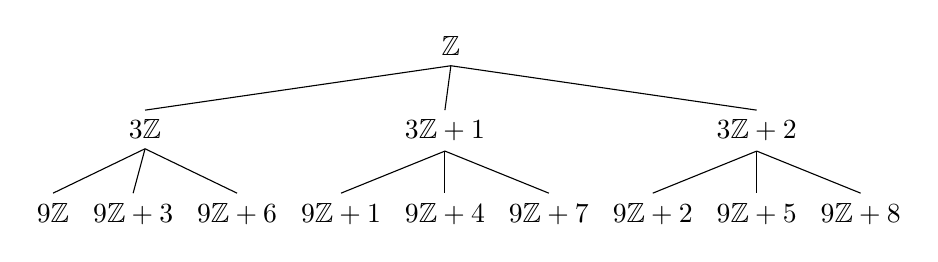
\begin{tikzpicture}
\Tree [. $\mathbb{Z}$  [. $3\mathbb{Z}$ [. $9\mathbb{Z}$ ] 
						   [. $9\mathbb{Z}+3$  ] 
						   [. $9\mathbb{Z}+6$ ] ] 
			      [. $3\mathbb{Z}+1$ [. $9\mathbb{Z}+1$ ] 
						        [. $9\mathbb{Z}+4$ ] 
						        [. $9\mathbb{Z}+7$ ] ] 
		 	      [. $3\mathbb{Z}+2$  [. $9\mathbb{Z}+2$ ] 
                                                                        [. $9\mathbb{Z}+5$ ] 
                                                                       [. $9\mathbb{Z}+8$ ] ] ] 
\end{tikzpicture}
\end{center}




We start by finding a $\rho_0$-ordering of $S_{\gamma_0}$, but this is trival since $S_{\gamma_0}$ has only a single element. Let us pick $0$ to be our choice on centre for $B^0_1=B(0,1)=\mathbb{Z}$. As we see from $T_S$, $S_{\gamma_0}$ is partitioned into $3$ closed balls of radius $\gamma_1=\frac{1}{3}$, namely $3\mathbb{Z}, 3\mathbb{Z}+1$, and $3\mathbb{Z}+2$. A choice of centres is given by $0,1$, and $2$, so that $A_0$ becomes:

\[A_0=
 \begin{pmatrix}
0 \\
1  \\
2 
\end{pmatrix}
\]


To start the $\rho-$ordering, concatenate the rows to obtain $\{0,1,2\}$, and to continue it, make a choice of centres for each of the closed balls of radius $\gamma_2=\frac{1}{9}$ partitioning the sets $3\mathbb{Z}+i$, $i \in 0,1,2$. For example, $3\mathbb{Z} =  9\mathbb{Z} \cup 9\mathbb{Z}+3 \cup 9\mathbb{Z}+6$, so a choice of centres for $B^1_1$ is given by $\{0,3,6\}$. Making choices for the remaining elements, we obtain: 

\[A_1=
 \begin{pmatrix}
0 & 1 &  2 & \\
3 & 4 &  5 & \\
6 & 7 &  8 &
\end{pmatrix}
\]

To continue the $\rho-$ordering we concatenate the rows, $\{0,1,2,3,4,5,6,7,8\}$, which also gives the first row of $A_2$. The remaining rows are found by partitioning each of the closed balls of radius $\frac{1}{9}$ and again making a choice of centres:
\[A_2=
 \begin{pmatrix}
0 & 1 &  2 & 3 & 4 & 5 & 6 & 7 & 8 \\
9 & 10 &  11 & 12 & 13 & 14 & 15 & 16 & 17 \\
18 & 19 &  20 & 21 & 22 & 23 & 24 & 25 & 26 \\
\end{pmatrix}
\]

And so on. 
\end{example}

We are able to make two statements following this example. The first is that in starting the $\rho_3-$ordering, the fact that $S_{\gamma_0}$ had only a single element allowed us to get started for free. In fact,  all compact ultrametric spaces are bounded, so this is always the case. \\

The second takeaway is that we found the start of a $\rho-$ordering of $S=(\mathbb{Z}, \rho_3)$ was given by taking the integers starting at $0$ in their natural order. If we had continued building the ordering, we would have continued to find this. The fact that the natural ordering on the integers is a $\rho_p-$ordering, where $\rho_p$ is the $p-$adic metric for any prime $p$, is well known \cite{mb1}, but we give an alternate proof of it here:\\ 

\begin{corollary} 
Let $S$ be the ultrametric space $(\mathbb{Z}, \rho_p)$, where $\rho_p$ is  $p-$adic metric for any prime $p$. The a $\rho_p-$ordering of $S$ can be found by taking the integers, starting at $0$, in their natural order.
\end{corollary}

\begin{proof}
We prove the above by induction on $k$. First note that for any choice of prime, the elements of $S_{\gamma_1}$ are the cosets of $\mathbb{Z}$ modulo $p$, so that $A_1$ has $p$ columns. Since $\{0,1,2\ldots,p-1\}$ are distributed among each of these cosets, without loss of generality the first row of $A_1$ is given by $[0,1,2,\ldots, p-1]$ in order.\\

Now suppose that the first row of $A_k$ is given by $[0,1,2,\ldots,n]$ for $0 < k < k+1$. We show the first row of $A_{k+1}$, and therefore the first $n'$ elements in a $\rho_p-$ordering of $S$, where $n'$ is the column dimension of $A_{k+1}$, can be obtained as $[0,1,2,\ldots,n,n+1,\ldots,n']$. First note that each closed ball of radius $p^k = \gamma_k$ is in fact a coset of $\mathbb{Z}$ modulo $p^k$, of which there are $p$. Then for any $k$, $A_k$ is a matrix with $p^k$ columns and $p$ rows. In particular, $n=p^k-1$. Let $i \in \{0,1,\ldots,p^{k}-1\}$ be arbitrary. Then $i$ is in exactly one of the cosets of $\mathbb{Z}$ modulo $p^k$ and since the first row of $A_k$ is $[0,1,2,\ldots,p^k-1]$, it must have been chosen as our representative of this coset. If we split $p^k\mathbb{Z}+i$ into balls of radius $p^{k+1}$, we have \[p^k\mathbb{Z}+i = \bigcup_{j=0}^{p-1} p^{k+1}\mathbb{Z} + (p^kj + i) \]
since there will be $p$ elements in the partition, each of which will be equal to $i$ modulo $p^k$ and distinct modulo $p^{k+1}$. Then, there is a choice of centres such that the $i^{th}$ column of $A_{k}$ is \[[i,p^k +i, 2p^k +i,\ldots, (p-1)p^k +i]^T\]
filling this in for each $i$, we see that $A_k$ can be obtained as:
\[A_k=
 \begin{pmatrix}
0 & 1 &  2 & \ldots & p^k -1 \\
p^k & p^k+1 &  p^k+2 & \ldots & p^k+(p^k-1) \\
2p^k & 2p^k+1 &  2p^k+2 & \ldots & 2p^k+(p^k-1) \\
\vdots &  \vdots & \vdots & \ddots & \vdots \\
(p-1)p^k & (p-1)p^k +1 &  (p-1)p^k+2 & \ldots & (p-1)p^k+(p^k-1)
\end{pmatrix}
\]

Concatenating the rows, we see the first row of $A_{k+1}$ will be \[[0,1,2,\ldots,p^k-1,p^k,\ldots,p^{k+1}-1]\] as required. 
\end{proof}

\begin{example}
Let us now see an example where there is an uneven number of children between the vertices on a given level. Suppose $S=\mathbb{Z} \setminus 4\mathbb{Z}$, a subset of $(\mathbb{Z}, \rho_2)$. In this case, we have that $\Gamma_S=\{1, \frac{1}{2},\frac{1}{4},\frac{1}{8},\ldots \}$ and $T_s$ begins:

\begin{center}
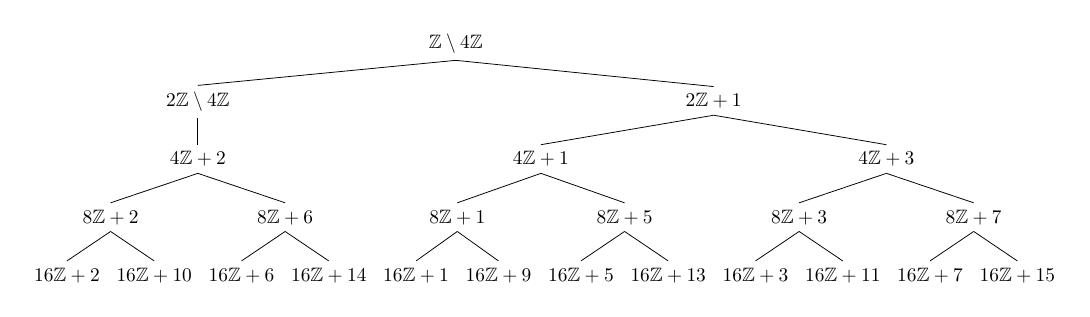
\begin{tikzpicture}[scale=.7]
\Tree [. $\mathbb{Z}\setminus 4\mathbb{Z}$  [. $2\mathbb{Z}\setminus 4\mathbb{Z}$  [. $4\mathbb{Z}+2$ [. $8\mathbb{Z}+2$ [. $16\mathbb{Z}+2$ ] [. $16\mathbb{Z}+10$ ] ] 
                                                            [. $8\mathbb{Z}+6$ [. $16\mathbb{Z}+6$ ] [. $16\mathbb{Z}+14$ ] ] ] ]
			                 [. $2\mathbb{Z}+1$ [. $4\mathbb{Z}+1$  [. $8\mathbb{Z}+1$ [. $16\mathbb{Z}+1$ ] [. $16\mathbb{Z}+9$ ] ]
			                                                        [. $8\mathbb{Z}+5$ [. $16\mathbb{Z}+5$ ] [. $16\mathbb{Z}+13$ ] ] ] 
			                                    [. $4\mathbb{Z}+3$  [. $8\mathbb{Z}+3$ [. $16\mathbb{Z}+3$ ] [. $16\mathbb{Z}+11$ ] ] 
			                                                        [. $8\mathbb{Z}+7$ [. $16\mathbb{Z}+7$ ] [. $16\mathbb{Z}+15$ ] ] ] ] ] 
\end{tikzpicture} 
\end{center}

Choosing centres for the partition of $\mathbb{Z}$ into closed balls of radius $\frac{1}{2}$, we have:
\[A_0=
 \begin{pmatrix}
2 \\
1  \\
\end{pmatrix}
\]

We have taken $S$ to be the complement of $4\mathbb{Z}$ in $\mathbb{Z}$, so $B(0,\gamma_1)$ has only one child, since $2\mathbb{Z} \setminus 4\mathbb{Z} = 4\mathbb{Z}+2$, while $B(1,\gamma_1)$ has two. Making a choice of centres, we have:

\[A_1=
 \begin{pmatrix}
2 & 1 \\
* & 3  \\
\end{pmatrix}
\]

We concatenate the rows, skipping over *, and again make a choice of centres for the closed balls of radius $\frac{1}{8}$:

\[A_1=
 \begin{pmatrix}
2 & 1 & 3 \\
6 & 5 & 7   \\
\end{pmatrix}
\]

One more iteration yields:

\[A_2=
 \begin{pmatrix}
2 & 1 & 3 & 6 & 5 & 7 \\
10 & 9 & 11 & 14 & 13 & 15   \\
\end{pmatrix}
\]

So that a $\rho_2-$ordering of $S=\mathbb{Z} \setminus 4\mathbb{Z}$ starts: $\{2,1,3,6,5,7,10,9,11,14,13,15,\ldots\}$.

\end{example}


%\begin{corollary}
%Interweaving the bottom row of the lattice of closed balls for a set $S$ gives a $\rho$-ordering of $S$. 
%\end{corollary}
In the two propositions above, there was notational difficulty that arose when there was an unequal number of children between the vertices on a given level of $T_s$. This difficulty is, in fact, more than a notational inconvenience, and the situation simplifies considerably when it is not the case. We are far from the first to observe this. Amice noted this as far back as her 1964 paper \cite{amice}, and it has been observed more recently by Chabert and colleagues, for example in \cite{fp} and \cite{cef}. The following section discusses this in more detail, first by supplying some preliminary lemmas and then showing how calculations are simplified in this setting.\\


\chapter{Application: Product spaces of $\mathbb{Z}_p$}
We consider now an application of the last two chapters. A natural space to consider is the product space of ultrametric spaces, for example $\mathbb{Z}^n$, for some $1 < n < \infty$. A natural candidate for an ultrametric on a finite product space is given by
\[ \rho_\infty(x,y) = \rho_\infty((x_1,x_2,\ldots,x_n),(y_1,y_2, \ldots, y_n)) = \max_{i} \{\rho(x_i, y_i)\}\] where $\rho$ is the metric from the base space.  We also see that no problems arise in letting both $M$ and $\rho$ vary between components of the space, as long as each $\rho_i$ is an ultrametric.

\begin{proposition}
Let $(M_i, \rho_i)$, for $i$ in some finite index set $I$, be a collection of metric spaces and suppose $\rho_i$ is an ultrametric for each $i$. Then $(M,\rho_\infty)$ is an ultrametric space, where $M=M_1 \times M_2 \times M_3 \times \ldots \times M_n$ and $\rho_\infty$ is the metric described above.
\end{proposition}

\begin{proof}
Let $(M, \rho_\infty)$ be the product of ultrametric spaces as above and let $x$ and $y$ be two points in the space. Clearly, $\rho_\infty(x,y) \geq 0$ since each $\rho_i(x_i,y_i) \geq 0$, and $\rho_\infty(x,y) = 0 \iff \rho_i(x_i,y_i) =0,\forall i \iff x_i=y_i, \forall i \iff x=y$. The fact that $\rho_\infty$ is symmetric is also an easy consequence of the fact that each $\rho_i$ is symmetric since  $\rho_i(x_i, y_i) = \rho_i(y_i, x_i)$ implies $\max_{i}\{\rho_i(x_i, y_i)\} = \max_i\{\rho_i(y_i, x_i)\}$. To see that $\rho_\infty$ is an ultrametric, note that if $z=\{z_i\}$ is any other point of $M$, then
\begin{align*}
   \qquad \rho_\infty(x, y)& = \max_i\{\rho_i(x_i,y_i)\}  \\
    &\leq \max_i\{\max(\rho_i(x_i,z_i),\rho_i(y_i,z_i))\} & \text{ since each $\rho_i$ is an ultrametric } \\
    &\leq \max(\max_i\{\rho_i(x_i,z_i)\}, \max_i\{\rho_i(y_i,z_i)\})  \\
    &= \max(\rho_\infty(x,z),\rho_\infty(y,z))  
\end{align*}
%* Let $M= max(sup_i(\{a_i\}, sup_j(\{b_j\})))$, then $M \geq a_i, \forall i$ and $M \geq b_i, \forall i$, so $M \geq max(a_i,b_i), \forall i$, hence $M \geq sup_i(max(a_i,b_i)$.
\end{proof}

If we are going to compute the capacity of product spaces, we must check that compactness is preserved when taking products. By Tychonoff's theorem, it is enough to show that the product metric, $\rho_\infty$, gives the product topology on the space. To do this, we adapt the proofs in Munkres (\cite{mun}), where they are given for the analogous case of finite products of $\mathbb{R}$.\\

\begin{definition-proposition} 
	(\cite{mun}, page 114) Suppose $X_i$, for $i$ in some index set $I$, is a family of topological spaces.  Let $\pi_j: \prod_{i \in I} X_i \rightarrow X_j$ be the map given by projection onto the $j$-th component, that is, $\pi_j (x) = \pi_j ((x_i)_{i \in I}) = x_j$. For each $j \in I$, let $\mathcal{S}_j$ be the collection \[\mathcal{S}_j = \{\pi^{-1}_j (U_j)\mid U_j \text{ open in } X_j\}\] Let $\mathcal{S}$ be the union of the $\mathcal{S}_j$ over $j \in I$, $\mathcal{S}= \cup_{j \in I} \mathcal{S}_j$. Then $\mathcal{S}$ is a subbasis that generates a topology on  $\prod_{i \in I} X_i$ called the \textbf{product topology}.\\
\end{definition-proposition}


The basis, $\mathcal{B}$, generated by $\mathcal{S}$ in the definition above is the set of all finite intersections of elements in $\mathcal{S}$. That is, $B \in \mathcal{B}$, if there exist $S_1, S_2, \ldots, S_n$ in $\mathcal{S}$ such that $B = S_1 \cap S_2 \cap \ldots S_n$.  A useful description of the basis for the product topology also appears in Munkres, as below:\\

\begin{proposition} 
	(\cite{mun}, Theorem 19.2) Suppose $X_i$, for $i$ in some index set $I$, is a family of topological spaces and denote by $\mathcal{B}_i$ the basis for the topology on $X_i$. Let 
	
	\begin{align*}
	\mathcal{B}_P = \prod_{i \in I} B_i, & \text{ for }  B_i \in \mathcal{B}_i \text { and } B_i = X_i \text{ for all but finitely-many } i \in I. 
	\end{align*}
	then $\mathcal{B}_P$ is a basis for the product topology on $\prod_{i \in I} X_i$.\\
	
\end{proposition}

We can now show that the topology induced by the $\rho_\infty$ metric described above agrees with the product topology for finite products.\\

\begin{proposition}
	Let $M=(M_{1} \times M_{2} \times \ldots \times M_{n},\rho_\infty)$ be a finite product of ultrametric spaces and let $\rho_\infty$ be the metric described above.  Then the topology induced by $\rho_\infty$ coincides with the product topology on $M_{1} \times M_{2} \times \ldots \times M_{n}$.
\end{proposition}

\begin{proof}
	(adpated from \cite{mun}, proof of Theorem 20.3) Let $\mathcal{T}_{\rho_\infty}$ be the topology on $M_{1} \times M_{2} \times \ldots \times M_{n}$ induced by $\rho_\infty$ and let $\mathcal{B}_{\rho_\infty}$ be the basis for this topology. Let $\mathcal{T}_{P}$ be the product topology with basis $\mathcal{B}_P$. We show $\mathcal{T}_{P} \subset \mathcal{T}_{\rho_\infty}$ and vice versa. For this, it is equivalent (\cite{mun}, Theorem 13.3) to show that for $z \in  M_{1} \times M_{2} \times \ldots \times M_{n}$ and $B \in \mathcal{B}_{P}$ containing $z$, there is a basis element $B' \in \mathcal{B}_{\rho_\infty}$ such that $z \in B' \subset B$, and vice versa.\\
	
	So let  $z \in M_{1} \times M_{2} \times \ldots \times M_{n}$ and suppose $B \in \mathcal{B}_{P}$ contains $z$. Since $B$ is in $\mathcal{B}_{P}$, $B$ is of the form $B(z_1,r_1) \times B(z_2,r_2) \times \ldots \times B(z_n,r_n)$ (since the choice of centres is arbitrary in an ultrametric space, we may choose the components of $z$ as the centres without loss of generality). Let $r=\min \{r_i\}$ for $i \in 1,\ldots, n$. Then let $B'$ be the ball $B(z,r)$ in $ \mathcal{B}_{\rho_\infty}$. Clearly, $z \in B(z,r)$ and since $r \leq r_i$, $\forall i$, $B(z,r) = B(z_1,r) \times B(z_2,r) \times \ldots \times B(z_n,r) \subset  B(z_1,r_1) \times B(z_2,r_2) \times \ldots \times B(z_n,r_n) =B$.\\
	
	Conversely, suppose $A \in \mathcal{B}_{\rho_\infty}$ and let $y \in A$. To find $A' \in \mathcal{B}_{P}$ such that $y \in A'$ and $A' \subset A$, simply note that $A$ itself is in $\mathcal{B}_{P}$.
	
\end{proof}

We are now ready to explore the capacity in these spaces. We first show that translation invariance carries over into product spaces under the expected conditions.\\ 

\begin{proposition}
Suppose $(M,\rho_\infty)$ is the product of ultrametric spaces $(M_i, \rho_i)$ and each $M_i$ is a topological group with operation $+_i$. Let $+$ denote the operation on $M$ given by $s+x = (s_1 + _1 x_1, s_2 +_2 x_2, \ldots, s_n +_nx_n)$ for $s = (s_1,\ldots,s_n)$ and $x =(x_1,\ldots,x_n)$ in $(M, \rho_\infty)$. Then $\rho_\infty$ is (left) translation invariant under $+$ if each $\rho_i$ is (left) translation invariant under $+_i$, in which case valuative capacity is also (left) translation invariant.
\end{proposition}

\begin{proof}
Let $(M,\rho_\infty)$ be as above. Suppose also that \[\rho_i(x_i,y_i) = \rho_i(s_i +_i x_i, s_i +_iy_i), \forall s_i, x_i, y_i \in M_i, \forall i.\] that is, suppose each $\rho_i$ is (left) translation invariant. Then,  
\begin{align*}
\rho_\infty(s +x, s+y) &= \max_i\{\rho_i(s_i +_ix_i, s_i +_i y_i)\} \\
&= \max_i\{\rho_i(x_i, y_i)\}\\
&= \rho_\infty(x,y).
\end{align*} 
so that $\rho_\infty$ is translation invariant.  Proposition \ref{translation invariance} implies that valuative capacity is as well. 
\end{proof}

In the next proposition, we show that scaling carries over to product space as well, although the conditions are now more restrictive. In contrast to the proposition above, here  we cannot allow the spaces to vary between components.\\

\begin{proposition}
Let $(m, \rho_N)$ be an ultrametric space, where $\rho_N$ is the metric induced by some norm $N$. Let $(M, \rho_{\infty})$ be the ultrametric space formed by taking products of $m$, along with the $\rho_\infty$ metric defined above.  Then if $\rho_N$ is multiplicative on $m$, $\rho_{\infty}$ is multiplicative on $M$, in the sense that $\rho_{\infty}(cx,cy) = \lvert c\rvert_{\rho_N} \text{ } \rho_\infty (x,y)$, for $c=(c,c,c,\ldots), x,y \in M$.
\end{proposition}

\begin{proof}
Let $M, \rho,$ and $\rho_{\infty}$ be as above. Then, 
\begin{align*}
\rho_\infty(cx, cy) &= \max_i\{\rho_N(c_i x_i, c_i y_i)\} \\
&= \max_i\{\vert c \rvert_{\rho_N} \text{ }  \rho_N(x_i, y_i)\} \\
&= \vert c \rvert_{\rho_N} \text{ } \max_i\{\rho_N(x_i,y_i)\} \\
&= \vert c \rvert_{\rho_N} \text{ } \rho_\infty(x_i,y_i)
\end{align*}
\end{proof}

\begin{corollary}
Let $S$ be a subset of $(M, \rho_\infty)$, where $M$ is the product of an ultrametric space $(m, \rho_N)$, which is itself a normed vector space with a multiplicative norm inducing $\rho_N$. If $c=(c,c,c,\ldots)$ is an element of $M$ with constant value on each component, then $\omega(cS)=\lvert c \rvert_{\rho_N} \text{ }\omega(S)$.
\end{corollary}

\begin{proof} 
The result follows by noting that if $\{a_j\}_{j=0}^\infty$ is a $\rho_\infty$ ordering of $S$, then $\{ca_j\}_{j=0}^\infty$ is a $\rho_\infty$ ordering of $cS$.
\end{proof}

We now introduce two examples, the details of which make up the rest of this chapter.\\ 

\begin{example}
	Let $(\mathbb{Z}_p \times \mathbb{Z}_p, \rho_{p,\infty})$ be the metric space with elements $\{(x,y)\mid x,y \in \mathbb{Z}\}$ and metric $\rho_{p,\infty}((x_1,x_2), (y_1,y_2)) = \max(\rho_p(x_1, y_1)), \rho_p(x_2, y_2))$, where $\rho_p$ is the p-adic metric for some fixed prime $p$. Since $\rho_p$ is translation invariant and multiplicative, valuative capacity is also translation invariant and multiplicative in  $(\mathbb{Z}_p \times \mathbb{Z}_p, \rho_{p,\infty})$.
\end{example}

\begin{example}
	Let $(\mathbb{Z}_{p_1} \times \mathbb{Z}_{p_2}, \rho_{P,\infty})$ be the metric space with elements $\{(x,y)\mid x,y \in \mathbb{Z}\}$ and metric $\rho_{P,\infty}((x_1,x_2), (y_1,y_2)) = \max(\rho_{p_1}(x_1, y_1)), \rho_{p_2}(x_2, y_2))$, for two distinct primes, $p_1 \neq p_2$, where both $\rho_{p_i}$ are p-adic metrics. Since each $\rho_{p_i}$ is translation invariant in $\mathbb{Z}$, valuative capacity will be translation invariant  in  $(\mathbb{Z}_{p_1} \times \mathbb{Z}_{p_2}, \rho_{P,\infty})$; however, unlike the case of $p_1=p_2$, this space does not have a multiplicative property that allows for scaling.
\end{example}

What is the valuative capacity of  $(\mathbb{Z}_p \times \mathbb{Z}_p, \rho_{p,\infty})$  from Example 12? Suppose $p=2$.  Using translation invariance, scaling and subaddivity, we can compute the result by first noting that we can write $\mathbb{Z}_2 \times \mathbb{Z}_2$ as a union, as below,\\
\[
\mathbb{Z}_2 \times \mathbb{Z}_2 = (2\mathbb{Z}_2 \times 2\mathbb{Z}_2) \cup (2\mathbb{Z}_2 \times 2\mathbb{Z}_2 +1) \cup (2\mathbb{Z}_2+1 \times 2\mathbb{Z}_2) \cup (2\mathbb{Z}_2+1, 2\mathbb{Z}_2+1).
\]

Since the pairwise distances on the right-hand side are always $1 = diam(\mathbb{Z}_2 \times \mathbb{Z}_2)$, the decomposition formula implies that \\

\begin{align*}
\qquad  \frac{1}{\log(\omega(\mathbb{Z}_2 \times \mathbb{Z}_2))}& = \frac{1}{\log(\omega(2\mathbb{Z}_2 \times 2\mathbb{Z}_2))} + \frac{1}{\log(\omega(2\mathbb{Z}_2 \times 2\mathbb{Z}_2 +1))} \\
  &\qquad \qquad + \frac{1}{\log(\omega(2\mathbb{Z}_2+1 \times 2\mathbb{Z}_2))} + \frac{1}{\log(\omega(2\mathbb{Z}_2+1 \times 2\mathbb{Z}_2+1))}\\
& = \frac{4}{\log(\lvert 2 \rvert_2 \cdot \omega(\mathbb{Z}_2 \times \mathbb{Z}_2))} \\
&= \frac{4}{\log(\frac{1}{2} \cdot \omega(\mathbb{Z}_2 \times \mathbb{Z}_2))}
% =  \frac{4}{log(\frac{1}{2}) + log(\omega(\mathbb{Z}_2 \times \mathbb{Z}_2))}\]
\end{align*}
Then,
\[4\cdot \log(\omega(\mathbb{Z}_2 \times \mathbb{Z}_2)) =\log(\frac{\omega(\mathbb{Z}_2 \times \mathbb{Z}_2)}{2}) \]


% Taking logs base $2$, we have that 
%\[\omega(\mathbb{Z}_2 \times \mathbb{Z}_2) = 2^{\frac{-1 + log_2(\omega(\mathbb{Z}_2 \times \mathbb{Z}_2))}{4}} =  2^{\frac{-1}{4}} 2^ {\frac{log_2(\omega(\mathbb{Z}_2 \times \mathbb{Z}_2))}{4}}
%= 2^{\frac{-1}{4}}{(2^ {log_2(\omega(\mathbb{Z}_2 \times \mathbb{Z}_2))})}^{\frac{1}{4}} = 2^{\frac{-1}{4}}{\omega(\mathbb{Z}_2 \times \mathbb{Z}_2)}^{\frac{1}{4}} \]

so that ${\omega(\mathbb{Z}_2 \times \mathbb{Z}_2)}$ is a solution of the equation $x^4 - \frac{x}{2}$, for which there is a single real positive root, given by $2^{-1/3}$.\\


To compute the valuative capacity for a $2$-fold product for an arbitary prime $p$, note that we can always decompose $\mathbb{Z}_p \times \mathbb{Z}_p$ into a union of $p^2$ sets, each of the form $\{(p\mathbb{Z}_p+s) \times (p\mathbb{Z}_p +t)\}$ for $s,t \in (0,\ldots, p-1)$, and the pairwise distance between these sets will always be $1 = diam(\mathbb{Z}_p \times \mathbb{Z}_p)$. (To see this, either note that we can always find co-prime elements, or note that each set is a closed ball of radius $1/p$ centred at (s,t) and so the distance between them must be greater than $1/p$, and $1$ is the only possible distance greater than $1/p$ in $\mathbb{Z}_p \times \mathbb{Z}_p$).  Then, we combine our tools as before to obtain the equation,\\

\[\frac{1}{\log(\omega(\mathbb{Z}_p \times \mathbb{Z}_p))} = \frac{p^2}{\log(\lvert p \rvert_p \cdot \omega(\mathbb{Z}_p \times \mathbb{Z}_p))} =  \frac{p^2}{\log(\frac{1}{p} \cdot \omega(\mathbb{Z}_p \times \mathbb{Z}_p))}    \]

In turn, we have 

\[ \omega(\mathbb{Z}_p \times \mathbb{Z}_p)^{p^2} =  \frac{\omega(\mathbb{Z}_p \times \mathbb{Z}_p)}{p}  \]

So that $\omega(\mathbb{Z}_p \times \mathbb{Z}_p)$ is a solution of the equation $x^{p^2} - \frac{x}{p} = x(x^{p^2-1} - \frac{1}{p})=0$ over $\mathbb{R}$. Since $\mathbb{R}$ is a field, this means the positive solutions are given by solving $x^{p^2-1}-\frac{1}{p}$. Solutions of this equation are of the form $p^{\frac{-1}{p^2-1}}$ times a $p^2-1$ root of unity, and so there is exactly one positive, real solution, namely $p^{\frac{-1}{p^2-1}}$ itself. Thus the valuative capacity of the entire product space $\mathbb{Z}_p \times \mathbb{Z}_p$ is $p^{\frac{-1}{p^2-1}}$. In fact, from here it is not hard to see that by taking the $n$-fold product, we would end up with the same equation except that the exponent of $p$ would become $n$ rather than $2$. We arrive at the following result:\\

\begin{proposition}
Let $M=(\mathbb{Z}_p^n, \rho_{p, \infty})$ be the ultrametric space with points equal to the $n$-fold product of $(\mathbb{Z}, \rho_p)$ (for $n < \infty$) for some fixed prime $p$. The valuative capacity of $M$ is  $(\frac{1}{p})^{\frac{1}{p^n-1}}$.
\end{proposition}

\begin{proof}
Above.
\end{proof}

Taking $n=1$, we see that this agrees with the valuative capacity of $\mathbb{Z}$ computed in the second chapter. \\

What about $(\mathbb{Z}_{p_1} \times \mathbb{Z}_{p_2})$ for distinct primes? These spaces do not admit a scaling property, so the same toolset is not available. They are, however, semi-regular, so we know that\\  \[v_{\gamma_k}(\sigma(n)) =  \lfloor\frac{n}{\beta(k)}\rfloor - \lfloor\frac{n}{\beta(k+1)}\rfloor = \sum_{j=1}^{\alpha(k)-1} \lfloor \frac{n + j\cdot \beta(k)}{\alpha(k)\beta(k)} \rfloor \]
Suppose $p_1 =2$ and $p_2 =3$. Recall that the $\alpha$ sequence of $S=(\mathbb{Z}_{2} \times \mathbb{Z}_{3})$ counts the number of closed balls of radius $\gamma_{k+1}$ partitioning a closed ball of radius $\gamma_k$. In this case, $\Gamma_S$ is the non-positive powers of $2$ and $3$ sorted into decreasing order, so that $\Gamma_S$ starts $\{1, \frac{1}{2},\frac{1}{3},\frac{1}{4},\frac{1}{8},\frac{1}{9},\ldots \}$ and $\alpha(S)$ starts $\{6,2,3,2,2,3,2,3,2,\ldots\}$. The $\beta$ sequence of $S$, which counts the number of distinct balls of a fixed radius, then starts $\{6,12,36,72,144,\ldots\}$.\\

We know that the capacity of $S$ will be a product of some negative power of $2$ and some negative power of $3$.  From Lemma \ref{semi-regular formula}, we know that when $\alpha(k)=2$, we have\\ 
\[v_{\gamma_k}(\delta(n)) = \lfloor \frac{n + \beta(k)}{2\cdot \beta(k)} \rfloor\]

and when $\alpha(k)=3$, we have\\
\[v_{\gamma_k}(\delta(n)) = \lfloor \frac{n + \beta(k)}{3\cdot \beta(k)} \rfloor + \lfloor \frac{n + 2\cdot \beta(k)}{3\cdot \beta(k)} \rfloor \]

We also know that if $\alpha(k)=2$, then $\gamma_k$ must be a (negative) power of $2$, and likewise if $\alpha(k)=3$, then $\gamma_k$ is a power of $3$.\\

Let us first explore the exponent of $2$ in $\delta(n)$. We start by noting that if $\gamma_k$ is some $2^{-i}$, then \[v_{\gamma_k}(\delta(n)) =\lfloor \frac{n + 2^i\cdot 3 ^j}{2^{i+1} \cdot 3^j} \rfloor \] since there will be a copy of $2$ in $\beta(k)$ for every occurence of $2$ in $\alpha(0),\ldots,\alpha(k)$, which is also what $i$ counts. So then, the exponent of $\frac{1}{2}$ in the $n^{th}$ characteristic sequence of $S$ is \[ \sum_{i=1}^\infty i \cdot \lfloor\frac{n + 2^i \cdot 3^j}{2^{i+1}\cdot 3^j} \rfloor\] What can we say about $j$, the exponent of $3$?\\ 

\begin{lemma}
Let $S = (\mathbb{Z}_{2} \times \mathbb{Z}_{3}) $ and consider the $k^{th}$ element of the $\beta$ sequence of $S$, $\beta(k) = 2^i \cdot 3^j$. If $k$ is such that $\gamma_k=2^{-i}$ for some $i$, then $j$ counts the numbers $a \in \mathbb{Z}_{\geq 0}$ such that $3^a < 2^{i}$.
\end{lemma}

\begin{proof}
$\Gamma_S$ is strictly monotone decreasing and each $\gamma_k$ is equal to a non-positive power of $2$ or $3$. If $\gamma_k = 2^i$, then all non-positive powers of $3$ and $2$ which are greater than $2^i$ must be equal to some $\gamma_j$, $0 \leq j < k$. That is, $2^i$ only appears in the $\Gamma_S$ sequence after all larger powers of $2$ and $3$ have been exhausted. Since we are only considering the case $\gamma_k$ is a power of $2$, this includes all of the smaller powers of~$3$.
\end{proof}

 Now note that\\ 
\begin{align*}
3^a < 2^i
 \iff
 \log_2(3^a) < \log_2(2^i)
\iff  
a \cdot \log_2(3) < i
\end{align*}

So now we are reduced to counting the number of non-negative integers $a$ that satisfy this last inequality for a given $i$.  The number of such $a$'s will simply be the the value of the largest $a$ plus $1$ since $a$ satisfying the relation implies all $0 \leq a' \leq a$ solve the relation. Then, we are in fact reduced to finding the largest $a \in \mathbb{Z}$ that satisfies $a < \frac{i}{log_2(3)}$, but this is exactly $\lfloor \frac{i}{log_2(3)}\rfloor$. This in turn gives $j =  \lfloor \frac{i}{log_2(3)}\rfloor + 1= \lceil \frac{i}{log_2(3)}\rceil$, since $\frac{i}{log_2(3)}$ is never an integer. We now revisit our expression for the exponent of $\frac{1}{2}$ and substitute our new found value for $j$:\\

\begin{align} 
\sum_{i=1}^\infty i \cdot \lfloor\frac{n + 2^i \cdot 3^{\lceil \frac{i}{log_2(3)}\rceil}}{2^{i+1}\cdot 3^{\lceil \frac{i}{log_2(3)}\rceil}} \rfloor
=\sum_{i=1}^\infty i \cdot (\lfloor\frac{n}{2^i \cdot 3^{\lceil \frac{i}{log_2(3)}\rceil }}\rfloor -  \lfloor\frac{n}{2^{i+1}\cdot 3^{\lceil \frac{i}{log_2(3)}\rceil}} \rfloor)
\end{align}
% for n from 1 to 100 do
% evalf(Sum(x*floor((n*10000+2^x*3^ceil(x/log[2](3)))/(2^(x+1)*3^ceil(x/log[2](3)))), x = 1 .. infinity));
%end do;
%identity fun
%for n from 1 to 100 do
 %evalf(1/(n*100000)*Sum(x*floor((n*100000+2^x*3^ceil(x/log[2](3)))/(2^(x+1)*3^ceil(x/log[2](3)))), x = 1 .. infinity));
%end do;


%First, recall that in computing the valuative capacity of these spaces, we were ultimately reduced to finding solutions to polynomials of the form $x^{p^n} - \frac{x}{p}$ for some $n$ and for some $p$. The first observation is that these polynomials are $\mathbb{Z}$-valued on $p\mathbb{Z}$, that is, they are elements of $Int(p\mathbb{Z},\mathbb{Z})$. We might ask then, what sort of polynomials would arise in finding the valuative capacity of spaces such as $(\mathbb{Z}_2 \times \mathbb{Z}_3, \rho_\infty)$ or in computing the valuative capacity of infinite product spaces, such as $\mathbb{Z}_p \times \mathbb{Z}_p \times \mathbb{Z}_p \times \ldots$ for either some fixed prime $p$ or over each prime. \\

A symmetric argument shows that exponent of $\frac{1}{3}$ in the $n^{th}$ element of the $\rho_\infty-$sequence of $S$ is\\ 

\begin{align} 
\sum_{i=1}^\infty i \cdot (\lfloor\frac{n + 2^{\lceil \frac{i}{log_3(2)}\rceil} \cdot 3^i}{2^{\lceil \frac{i}{log_3(2)}\rceil}\cdot 3^{i+1}} \rfloor + \lfloor\frac{n + 2^{\lceil \frac{i}{log_3(2)}\rceil+1} \cdot 3^i}{2^{\lceil \frac{i}{log_3(2)}\rceil}\cdot 3^{i+1}} \rfloor)
\end{align}

%\[=\sum_{i=1}^\infty i \cdot (\lfloor\frac{n}{2^{\lceil \frac{i}{log_3(2)}\rceil } \cdot 3^i}\rfloor -  \lfloor\frac{n}{2^{\lceil \frac{i}{log_3(2)}\rceil}\cdot 3^{i+1}} \rfloor)\]

The sums that appear in $(5.1)$ and $(5.2)$ are real numbers that we, at present, know  little about. However, the aperiodicity of the sequences $\lceil\frac{i}{log_2(3)}\rceil$ and $\lceil\frac{i}{log_3(2)}\rceil$ over $i$ leads us to believe, but not prove, that each of the sums are irrational. We have the following conjecture.\\

\begin{conjecture} Finite products of $(\mathbb{Z}, \rho_{p_i})$ for distinct primes, $p_i$, have transcendental valuative capacity.\\ \end{conjecture}
 
What can we say about the \textit{infinite} product of either $\mathbb{Z}_{p}$, for some fixed prime $p$ or $\mathbb{Z}_{p_i}$ for each prime? For a fixed prime $p$,  we can observe that $(\frac{1}{p})^{\frac{1}{p^n-1}}$ is a monotone, increasing sequence in $n$ with $ lim_{n\to\infty} (\frac{1}{p})^{\frac{1}{p^n-1}} =  1$ and in fact, the sequence $\{(0,0,\ldots), (1,0,\ldots), (0,1,\ldots), \ldots\}$, in which the first element has only zeros and the $n$-th element has a single $1$ in the $(n-1)$-th component, is a $\rho-$ordering. This might lead us to wonder if valuative capacity can obtain the diameter of the space. We are immediately met with a problem however.\\

Compactness has played no small role in this work. Indeed, we have a definition of valuative capacity only for compact subsets. 
We are now naturally left to ask whether the product topology on \textit{infinite} products of ultrametric spaces coincides with the $\rho_\infty$ metric. In this case, as in the analogous case of infinite copies of $\mathbb{R}$ and a uniform metric, the answer is negative (at least in general). Although, we can find a metric that realizes the product topology on infinite copies of ultrametric spaces (adapting the analogous case from copies of $\mathbb{R}$), there is nothing canonical about this construction. Although this is, on the one hand, a disappointment, on the other hand, it suggests a new avenue to explore: can we define valuative capacity for locally compact spaces, and if so, is capacity computable for any of these spaces?


%\textul{Example from previous chapter with more detail}:

\begin{example}
Consider the ultrametric space $(\mathbb{Z}, \rvert \cdot \lvert_p)$  for any prime $p$. Then $\beta(k)=p^k$ and $\alpha(k)=p$ for any $k$. The above gives 
\[v_{\gamma_k}(\sigma(n)) =\lfloor \frac{n}{p^{k}}\rfloor - \lfloor \frac{n}{p^{k+1}} \rfloor\]
and since $\gamma_k = p^{-k}$, $\forall k$, we have 
\[v_{\frac{1}{p}}(\sigma(n)) \]
\[ = \sum_{k=1}^{\infty} k \cdot (\lfloor \frac{n}{p^{k}}\rfloor - \lfloor \frac{n}{p^{k+1}} \rfloor) \]
\[ = \sum_{k=1}^{\lceil log_p(n) \rceil}  k \cdot (\lfloor \frac{n}{p^{k}}\rfloor - \lfloor \frac{n}{p^{k+1}} \rfloor)\]
\[ = \lfloor \frac{n}{p}\rfloor - \lfloor \frac{n}{p^{2}} \rfloor +  2\lfloor \frac{n}{p^2}\rfloor - 2\lfloor \frac{n}{p^3} \rfloor + \ldots +  \lceil log_p(n)\rceil \lfloor \frac{n}{p^{ \lceil log_p(n)\rceil}} \rfloor \]
\[ = \lfloor \frac{n}{p}\rfloor + \lfloor \frac{n}{p^2}\rfloor  + \ldots +  \lfloor \frac{n}{p^{ \lceil log_p(n)\rceil}} \rfloor \]
\[ =  \sum_{k=1}^{\lceil log_p(n) \rceil} \lfloor \frac{n}{p^{k}}\rfloor \]
\[ =  \sum_{k=1}^{\infty} \lfloor \frac{n}{p^{k}}\rfloor \]
\[= v_{p}(n!) \]

since $\lfloor \frac{n}{p^k} \rfloor = 0$ if $ p^k > n \iff log(p^k) > log(n) \iff k > log_p(n)$
\end{example}


\textul{The 2-3 case}:

What about $(\mathbb{Z}_{p_1} \times \mathbb{Z}_{p_2})$ for distinct primes? These spaces do not admit a scaling property, so the same toolset is not available. They are however semi-regular, so we know that  \[v_{\gamma_k}(\sigma(n)) =  \lfloor\frac{n}{\beta(k)}\rfloor - \lfloor\frac{n}{\beta(k+1)}\rfloor = \sum_{j=1}^{\alpha(k)-1} \lfloor \frac{n + j\cdot \beta(k)}{\alpha(k)\beta(k)} \rfloor \]
Suppose $p_1 =2$ and $p_2 =3$, so that the $\alpha$ sequence of $S = (\mathbb{Z}_{2} \times \mathbb{Z}_{3})$ is $\alpha = \{6,2,3,2,2,3,2,3,2,\ldots\}$ and the $\beta$ sequence is then $\beta = \{6,12,36,72,144,\ldots\}$. We know that the capacity of $S$ will be a product of some negative power of $2$ and a negative power of $3$.  From the above, we know that when $\alpha(k)=2$, we have 
\[v_{\gamma_k}(\sigma(n)) = \lfloor \frac{n + \beta(k)}{2\cdot \beta(k)} \rfloor\]

and when $\alpha(k)=3$, we have
\[v_{\gamma_k}(\sigma(n)) = \lfloor \frac{n + \beta(k)}{3\cdot \beta(k)} \rfloor + \lfloor \frac{n + 2\cdot \beta(k)}{3\cdot \beta(k)} \rfloor \]

We also know that if $\alpha(k)=2$, then $\gamma_k$ must be a (negative) power of $2$, and likewise if $\alpha(k)=3$, then $\gamma_k$ is a power of $3$.\\

 Let us first explore the exponent of $2$ in $\sigma(n)$. We start by noting that if $\gamma_k$ is some $2^{-i}$, then \[v_{\gamma_k}(\sigma(n)) =\lfloor \frac{n + 2^i\cdot 3 ^j}{2^{i+1} \cdot 3^j} \rfloor \] since there will be a copy of $2$ in $\beta(k)$ for every occurence of $2$ in $\alpha(0),\ldots,\alpha(k)$, which is also what $i$ counts. So then, the exponent of $\frac{1}{2}$ in the $n^{th}$ characteristic sequence of $S$ is \[ \sum_{i=1}^\infty i \cdot \lfloor\frac{n + 2^i \cdot 3^j}{2^{i+1}\cdot 3^j} \rfloor\] What can we say about $j$, the exponent of $3$? 

\begin{lemma*}
Let $S = (\mathbb{Z}_{2} \times \mathbb{Z}_{3}) $ and consider the $k^{th}$ element of the $\beta$ sequence of $S$, $\beta(k) = 2^i \cdot 3^j$. If $k$ is such that $\gamma_k=2^{-i}$ for some $i$, then $j$ counts the numbers $a$ in $\mathbb{Z}_{\geq 0}$ such that $3^a < 2^{i}$.
\end{lemma*}

\begin{proof}
(sketch) $2^i$ only makes it into the sequence after all smaller powers of $3$ and $2$ have been used, and since we are only considering the case $\gamma_k$ is a power of $2$, we get all the smaller powers of $3$.
\end{proof}

 Now note that  
\begin{align}
3^a < 2^i
 \iff
 log_2(3^a) < log_2(2^i)
\iff  
a \cdot log_2(3) < i
\end{align}

So now we are reduced to counting the number of non-negative integers $a$ that satisfy the above for a given $i$.  Note that the number of such $a$'s will simply be the the value of the largest $a$ plus $1$ since $a$ satisfying the relation implies all $0 \leq a' \leq a$ solve the relation. Then, we are in fact reduced to finding the largest $a \in \mathbb{Z}$ that satisfies $a < \frac{i}{log_2(3)}$, but this is exactly $\lfloor \frac{i}{log_2(3)}\rfloor$. This in turn gives $j =  \lfloor \frac{i}{log_2(3)}\rfloor + 1= \lceil \frac{i}{log_2(3)}\rceil$, since $\frac{i}{log_2(3)}$ is never an integer. We now revisit our expression for the exponent of $\frac{1}{2}$ and substitute our new found value for $j$:
 
\[\sum_{i=1}^\infty i \cdot \lfloor\frac{n + 2^i \cdot 3^{\lceil \frac{i}{log_2(3)}\rceil}}{2^{i+1}\cdot 3^{\lceil \frac{i}{log_2(3)}\rceil}} \rfloor\]
\[=\sum_{i=1}^\infty i \cdot (\lfloor\frac{n}{2^i \cdot 3^{\lceil \frac{i}{log_2(3)}\rceil }}\rfloor -  \lfloor\frac{n}{2^{i+1}\cdot 3^{\lceil \frac{i}{log_2(3)}\rceil}} \rfloor)\]
%S :=Sum(x*(floor((n + 2^x*3^ceil(x/log[2](3)))/(2^(x+1)*3^ceil(x/log[2](3))))), x=1..100)





%\chapter*{nov_presentation}
%\documentclass{beamer}
%\usepackage[utf8]{inputenc}
\usepackage{graphicx}
%\usepackage{tgtermes} 
\graphicspath{ {images/} }
\usepackage{mathtools}
\usepackage{amssymb}
\usepackage{amsfonts}
\usepackage{fancyvrb}
\usepackage{tikz}
\usepackage{tikz-qtree}
\usepackage{listings}
\usepackage{multicol}
\usepackage{amsthm}
\usepackage{amsmath }
\usepackage{xcolor}
\usepackage{framed}
\usepackage{color,soul}
\usepackage{tikz-cd}
\usetikzlibrary{matrix,arrows,decorations.pathmorphing, shadows, trees}
\usepackage{nomencl}
\usepackage{geometry}
\usepackage{setspace}
\usepackage{enumerate}



\theoremstyle{definition}
\newtheorem{proposition}{Proposition}
\newtheorem*{proposition*}{Proposition}
\newtheorem{definition_proposition}{Definition-Proposition}
\newtheorem*{definition_proposition*}{Definition-Proposition}
\newtheorem*{lemma*}{Lemma}
\newtheorem*{definition*}{Definition}
\newtheorem{conjecture}{Conjecture}

\title{Valuative capacity of compact subsets of ultrametric spaces}
\author{Anne Johnson}
\date{August 9, 2019}



\begin{document}
\maketitle

\begin{frame}{Background}
\begin{definition}	
(\cite{fek}) Let $K \subseteq \mathbb{C}$ be a compact subset. Fix $n \in \mathbb{N}$, and for $z = (z_1,\ldots,z_n) \in K^n$, consider
\[\delta_n(z) = \prod_{j < i} \lvert z_i - z_j \rvert^{\frac{2}{(n(n-1))}} \]
An element $z = (z_1,\ldots,z_n) \in K^n$ is called a \textbf{Fekete n-tuple} if $z$ maximizes $\delta_n$ over all $n-$tuples in $K$.
\end{definition}
%Note to self: do an example with 5 charged particles in a conductor
%Note to self: this cannot be done recursively
\end{frame}

\begin{frame}{Background}
	\begin{definition}	
		\cite{fek} Let $K$ be a compact subset of a metric space, $(M,\rho)$. Fix $n \in \mathbb{N}$, and for $z = (z_1,\ldots,z_n) \in K^n$, consider
		\[\delta_n(z) = \prod_{j < i} \rho(z_i, z_j)^{\frac{2}{(n(n-1))}} \]
		An element $z = (z_1,\ldots,z_n) \in K^n$ is called a \textbf{generalized Fekete n-tuple} if $z$ maximizes $\delta_n$ over all $n-$tuples in $K$.
	\end{definition}
\end{frame}

\begin{frame}{Background}
 \begin{definition}
		(\cite{mb1}) Let $S$ be a subset of $\mathbb{Z}$  and let $p$ be any prime. A \textbf{$p$-ordering} of $S$ is a sequence, $\{a_i\}_{i\geq 0}$ in $S$, such that $a_0$ is arbitrary and for $i >0$, $a_i$ minimizes 
		\[ v_p (\prod_{j < i} (z - a_j) )\] over $z \in S$.\\
 \end{definition}
	\pause
 \begin{itemize}
		\item $p-$orderings give a recursive construction for generalized Fekete $n-$tuples\only<+>{.}\only<+->{!}  
 \end{itemize}	
\end{frame}

\begin{frame}{Background}
\begin{definition}	
	(\cite{fek})Let $K \subseteq \mathbb{C}$ be a compact subset. The \textbf{transfinite diameter} of $K$ is \[ \lim_{n\to\infty} [ \max_z \text{ } \delta_n(z)]\] where the maximum is taken over all $n-$tuples in $K$. %That is, the transfinite diameter of $K$ is $ \lim_{n\to\infty} \delta_n(z)$, where $z$ is a Fekete $n-$tuple for each $n$.
\end{definition}
%Note to self: the convergence of this expression is Fekete's lemma
\end{frame}

\begin{frame}{Background}
\begin{proposition*}
	(\cite{jlc}, theorem 4.2)	Let $E$ be a subset of $V$, a rank-one valuation domain with valuation $v$. If $\{a_i\}_{i \geq 0}$ is $v-$ordering of $E$, then
	\[\lim_{n\to\infty} \frac{1}{n} \sum_{k=0}^{n-1} v(a_n-a_k) =\frac{2}{n(n+1)} \inf_{x_0, \ldots, x_n \in E} v (\prod_{0\leq j < i \leq n} (x_i-x_j))\]
\end{proposition*}
\end{frame}

\begin{frame}{Valuative capacity: set-up}
	\begin{definition}
		(\cite{kj}) Let $S$ be a compact subset of $(M,\rho)$. A \textbf{$\rho$-ordering} of $S$ is a sequence, $\{a_i\}_{i\geq 0}$ in $S$, such that $a_0$ is arbitrary and for $i >0$, $a_i$ maximizes 
		\[ \prod_{j < i} \rho(z, a_j) )\] over $z \in S$.\\
	\end{definition}
	\pause
    \begin{itemize}
	   \item If $\rho$ is an ultrametric, the terms $\prod_{i=0}^n \rho(a_n - a_j)$ do not depend on the choice of $\rho-$ordering. We call this the \textbf{$\rho-$sequence} of $S$. \\
	\end{itemize}
\end{frame}

\begin{frame}{Valuative capacity: set-up}
	\begin{itemize}
		\item $\rho-$orderings give a recursive construction for generalized Fekete $n-$tuples.\\	
		\pause	
		\item The limit \[ \omega(S):= \lim_{n\to\infty} [\prod_{i=0}^n \rho(a_n - a_j)]^{\frac{1}{n}}\] is called the \textbf{valuative capacity} of $S$.
	\end{itemize}		  
\end{frame}

\begin{frame}{Valuative capacity: facts}
Valuative capacity has the following properties:
\begin{itemize}
	\item \textit{translation-invariance}, i.e., $\omega(a+S) = \omega(S)$\\ (under a translation-invariant operation)
	\pause
	\item \textit{scaling}, i.e., $\omega(bS) = \lvert b\rvert \omega(S)$\\ (under a multiplicative norm)
	\pause
	\item \textit{decomposition}, i.e., \[\frac{1}{log(\frac{\omega(S)}{d}) } = \sum_{i=1}^n \frac{1}{log(\frac{\omega(A_i)}{d})}\]
	for $d=diam(S)$ and $\rho(A_i, A_j)=d, \forall i,j$ 
\end{itemize}	
\end{frame}

\begin{frame}{Recursive $\rho-$orderings}
	\tikzset{font=\tiny,
	level distance=1.35cm,
}

\begin{center}
	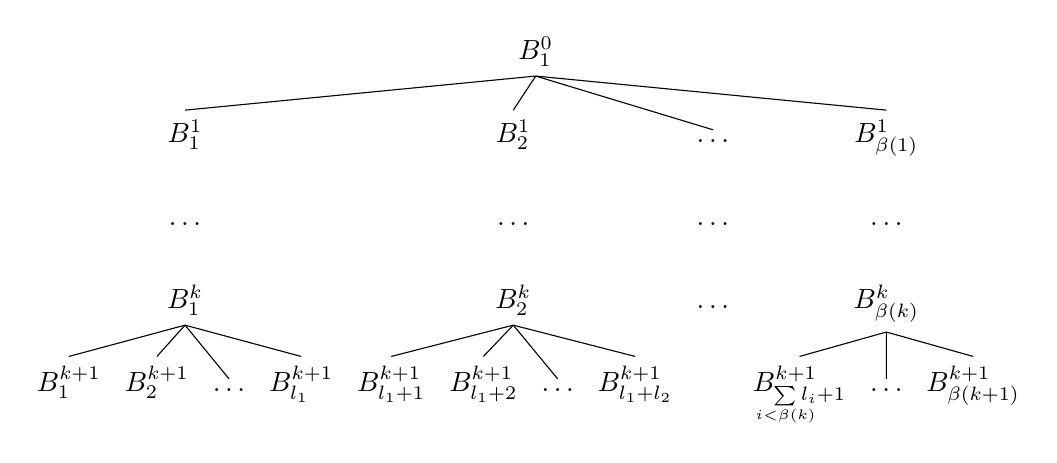
\begin{tikzpicture}
\Tree [. $B^0_1$ [. $B^1_1$ \edge [draw=none]; [. $\ldots$ \edge [draw=none]; [. $B^k_1$ [. $B^{k+1}_1$ ] [. $B^{k+1}_2$ ]  [. $\ldots$ ] [. $B^{k+1}_{l_1}$ ] ] ] ] 
[. $B^1_2$ \edge [draw=none]; [. $\ldots$ \edge [draw=none]; [. $B^k_2$ [. $B^{k+1}_{l_1 + 1}$ ] [. $B^{k+1}_{l_1 + 2}$ ] [. $\ldots$ ] [. $B^{k+1}_{l_1 + l_2}$ ] ] ] ] 
[. $\ldots$  \edge [draw=none]; [. $\ldots$ \edge [draw=none]; [. $\ldots$ ] ] ]
[.$B^1_{\beta(1)}$ \edge [draw=none]; [. $\ldots$ \edge [draw=none]; [.$B^k_{\beta(k)}$ [. $B^{k+1}_{\sum\limits_{\mathclap{i < \beta(k)}}  l_i + 1 }$ ] [. $\ldots$ ] [. $B^{k+1}_{\beta(k+1)}$ ] ] ] ] ]
\end{tikzpicture}
\end{center}
\end{frame}

\begin{frame}{Recursive $\rho$-orderings}
	
%Note to self: write notation on the board, $\Gamma_S$ and $\beta(k)$

	\begin{itemize}
		\item $\rho_{k+1}-$ordering of $S_{\gamma_{k+1}}$ is found by selecting elements of each $B^k_i$ in order as much as possible, and skipping to $B^k_{i+1}$, when it is not possible.
		\pause
		\item  to build a $\rho-$ordering of $S$ from the above, it suffices only to make a choice of centres for each of $B^k_i$'s.
	\end{itemize}
%Note to self: talk about shuffles
\end{frame}


\begin{frame}{Semi-regularity}
%Note to self: define semi-regularity	
\begin{proposition}
	If $S$ is a semi-regular ultrametric space, $\delta$ is the characteristic sequence of $S$, $\beta$ is the structure sequence of $S$, and $\alpha$ is the sequence describing the semi-regularity, then
	\[v_{\gamma_k}(\delta(n)) =  \lfloor\frac{n}{\beta(k)}\rfloor - \lfloor\frac{n}{\beta(k+1)}\rfloor = \sum_{j=1}^{\alpha(k)-1} \lfloor \frac{n + j\cdot \beta(k)}{\alpha(k)\beta(k)} \rfloor\]
\end{proposition}

\end{frame}


\begin{frame}{Regularity}
	%Note to self: define regularity
\begin{proposition}
	Let $S$ be a regular, tame subset of a compact ultrametric space with $\gamma_k = q^{c_k}$ for some $c_k \in \mathbb{Q}$ and for all $k \in \mathbb{N} \cup 0$. Then 
	\[v_{q}(\delta(n)) =  c_0n + \sum_{k=1}^{\infty} (c_{k} - c_{k-1}) \cdot \lfloor\frac{n}{q^{k}}\rfloor \]
	and 
	\[log_q(\omega(S)) = \lim_{n\to\infty} c_0 + \frac{1}{n}\sum_{k=1}^{\infty} (c_{k} - c_{k-1}) \cdot \lfloor\frac{n}{q^{k}}\rfloor  \]
\end{proposition}
\end{frame}

\begin{frame}
	\begin{itemize}
		\item  Semi-regularity implies the presence of a ``well-balanced" partition of $S$.
		\pause
		\item Regularity shows us that we can recover a notion of scaling, when the conditions are right.
		\pause 
		\item Taken together, they extend the toolkit for computing capacity without appealing to algebraic structure\only<+>{.}\only<+->{!} 
	\end{itemize}
\end{frame}


\begin{frame}{Product Space}
\begin{proposition}
	Let $(M_i, \rho_i)$, for $i$ in some finite index set $I$, be a collection of metric spaces and suppose $\rho_i$ is an ultrametric for each $i$. Then $(M,\rho_\infty)$ is an ultrametric space, where $M=M_1 \times M_2 \times \ldots \times M_n$ and $\rho_\infty$ is the metric described above.
\end{proposition}
\pause
\begin{itemize}
	\item Let $M=(\mathbb{Z}^n, \rho_{p, \infty})$ be the ultrametric space with points equal to the $n$-fold product of $(\mathbb{Z}, \rho_p)$ (for $n < \infty$) for some fixed prime $p$. The valuative capacity of $M$ is  $(\frac{1}{p})^{\frac{1}{p^n-1}}$.
	\pause
	\item What about primes $p \neq q$?
\end{itemize}
\end{frame}

\begin{frame}{Product Space: primes $p \neq q$}
	\begin{itemize}
		\item These spaces do not have a scaling property and they are not regular.
		\pause
		\item We use the fact that they are semi-regular and study the exponent of each prime in turn.
	\end{itemize}
\end{frame}

\begin{frame}{Product Space: $(\mathbb{Z},\rho_2) \times (\mathbb{Z},\rho_3)$}
\begin{lemma}
	Let $S = (\mathbb{Z},\rho_2) \times (\mathbb{Z},\rho_3) $ and consider the $k^{th}$ element of the $\beta$ sequence of $S$, $\beta(k) = 2^i \cdot 3^j$. If $k$ is such that $\gamma_k=2^{-i}$ for some $i$, then $j$ counts the numbers $a \in \mathbb{Z}_{\geq 0}$ such that $3^a < 2^{i}$.
\end{lemma}
\pause
\begin{proof}
	\begin{itemize}
	\item $\Gamma_S$ is strictly monotone decreasing and each $\gamma_k$ is equal to a non-positive power of $2$ or $3$. \pause
	\item If $\gamma_k = 2^i$, then all non-positive powers of $3$ and $2$ which are greater than $2^i$ must be equal to some $\gamma_j$, $0 \leq j < k$.\pause %That is, $2^i$ only appears in the $\Gamma_S$ sequence after all larger powers of $2$ and $3$ have been exhausted.
	\item Since we are only considering the case $\gamma_k$ is a power of $2$, this includes all of the smaller powers of $3$.
	\end{itemize}
\end{proof}
\end{frame}
\begin{frame}{Product Space: $(\mathbb{Z},\rho_2) \times (\mathbb{Z},\rho_3)$}
	 \[v_{\gamma_{\frac{1}{2}}}(\delta(n)) = \sum_{i=1}^\infty i \cdot \lfloor\frac{n + 2^i \cdot 3^{\lceil \frac{i}{log_2(3)}\rceil}}{2^{i+1}\cdot 3^{\lceil \frac{i}{log_2(3)}\rceil}} \rfloor\]
		\pause
	 \[v_{\gamma_{\frac{1}{3}}}(\delta(n)) = \sum_{i=1}^\infty i \cdot (\lfloor\frac{n + 2^{\lceil \frac{i}{log_3(2)}\rceil} \cdot 3^i}{2^{\lceil \frac{i}{log_3(2)}\rceil}\cdot 3^{i+1}} \rfloor + \lfloor\frac{n + 2^{\lceil \frac{i}{log_3(2)}\rceil+1} \cdot 3^i}{2^{\lceil \frac{i}{log_3(2)}\rceil}\cdot 3^{i+1}} \rfloor) \]
\end{frame}

\begin{frame}{Product Space: primes $p \neq q$}
\begin{conjecture} Finite products of $(\mathbb{Z}, \rho_{p_i})$ for distinct primes, $p_i$, have transcendental valuative capacity.\\ \end{conjecture}
\end{frame}


\begin{frame}
\frametitle{references}
\begin{thebibliography}{9}
%	\bibitem[Ac]{na} N.L. Ackerman, Completeness in Generalized Ultrametric Spaces, \textit{$p$-Adic Numbers, Ultrametric Analysis, and Applications} \textbf{5(2)} (2013), 89-105.
%	\bibitem[Am]{amice} Y. Amice, Interpolation $p$-adique, \textit{Bull. Soc. Math. France} \textbf{92} (1964) 117-180.
%	\bibitem[BR]{rum} M. Baker and R Rumely, \textit{Potential Theory and Dynamics on the Berkovich
%		Projective Line}, Amer. Math. Soc., Providence, 2010.
	\bibitem[B1]{mb2} M. Bhargava, $P$-orderings and polynomial functions on arbitrary subsets of Dedekind
	rings, \textit{J. reine angew. Math.}, \textbf{490} (1997), 101-127.
	\bibitem[B2]{mb1} M. Bhargava, The factorial function and generalizations, \textit{Am. Math. Monthly}
	\textbf{107} (2000), 783-799.
%	\bibitem[B3]{mb3} M. Bhargava, On $P$-orderings, Rings of Integer Valued Polynomials and Ultrametric
%	Analysis, \textit{Journal of the Amer. Math. Soc.} \textbf{22(4)} (2009), 963-993.
%	\bibitem[Ca]{dgc}  D. Cantor, On an extension of the definition of transfinite diameter and some applications, \textit{J. reine angew. Math} \textbf{316} (1980), 160-207.  
	\bibitem[Ch]{jlc} J.-L. Chabert, Generalized factorial ideals, \textit{Commutative algebra, Arab. J. Sci. Eng.
		Sect. C} \textbf{26} (2001), 51-68.
%	\bibitem[CEF]{cef} J.-L.Chabert, S. Evrard, Y. Fares, Regular subsets of valued fields and Bhargava’s $v$-orderings, \textit{Math. Z.} \textbf{274} (2013) 263-290.
%	\bibitem[EF]{ef} S. Evrard and Y. Fares, $p$-adic subsets whose factorials satisfy a generalized Legendre
%	formula, \textit{London Math. Soc.}, \textbf{40} (2008), 37-50.
%	\bibitem[FP]{fp} Y. Fares, S. Petite, The valuative capacity of subshifts of finite type, \textit{J. Number Theory} \textbf{158}
%	(2016), 165-184.
	%\bibitem[GV]{gvdp} Lothar Gerritzen and Marius van der Put, Schottky Groups and Mumford Curves.
	\bibitem[F]{fek} M. Fekete, Uber die Verteilung der Wurzelen bei gewisser algebraiche Gleichun-
	gen mit ganzzahligen Koeffizienten, \textit{Math. Zeits.} \textbf{17} (1923), 228-249.
	\bibitem[J1]{kj} K. Johnson, $p$-orderings, Fekete $n-$tuples and capacity in ultrametric spaces (in preparation).
%	\bibitem[J2]{kj2} K. Johnson, Limits of characteristic sequences of integer-valued polynomials on
%	homogeneous sets, \textit{J. Number Theory} \textbf{129} (2009), 2933-2942.
%	\bibitem[M]{mun} J. Munkres, \textit{Topology}, Prentice Hall Inc., Upper Saddle River NJ, 2000.
%	\bibitem[Ra1]{rand} T. Ransford, \textit{Potential Theory in the Complex Plane}, Cambridge University Press, Cambridge, 1995.
%	\bibitem[Ra2]{rand2} T. Randsford, Computation of Logarithmic Capacity, \textit{Comp. Methods Function Theory} \textbf{10} (2010), 555-578.
%	\bibitem[Ro]{ar} A.M. Robert, \textit{A course in p-adic analysis}, Springer-Verlag, New York, 2000.
%	\bibitem[S]{sim} B. Simon, Equilibrium measures and capacities in spectral theory, \textit{Inverse Probl. Imaging} \textbf{1}:4 (2007), 713–772. 
%	\bibitem[W]{wer} J. Wermer, \textit{Potential Theory}, Springer Lecture Notes in Mathematics, \textbf{408}, Providence, 1981.
\end{thebibliography}\end{frame}

\end{document}
%\chapter*{feb_presentation}
%\documentclass{beamer}
%\usepackage[utf8]{inputenc}
\usepackage{graphicx}
%\usepackage{tgtermes} 
\graphicspath{ {images/} }
\usepackage{mathtools}
\usepackage{amssymb}
\usepackage{amsfonts}
\usepackage{fancyvrb}
\usepackage{tikz}
\usepackage{tikz-qtree}
\usepackage{listings}
\usepackage{multicol}
\usepackage{amsthm}
\usepackage{amsmath }
\usepackage{xcolor}
\usepackage{framed}
\usepackage{color,soul}
\usepackage{tikz-cd}
\usetikzlibrary{matrix,arrows,decorations.pathmorphing, shadows, trees}
\usepackage{nomencl}
\usepackage{geometry}
\usepackage{setspace}
\usepackage{enumerate}



\theoremstyle{definition}
\newtheorem{proposition}{Proposition}
\newtheorem*{proposition*}{Proposition}
\newtheorem{definition_proposition}{Definition-Proposition}
\newtheorem*{definition_proposition*}{Definition-Proposition}
\newtheorem*{lemma*}{Lemma}
\newtheorem*{definition*}{Definition}
\newtheorem{conjecture}{Conjecture}

\title{Valuative capacity of compact subsets of ultrametric spaces}
\author{Anne Johnson}
\date{August 9, 2019}



\begin{document}
\maketitle

\begin{frame}{Background}
\begin{definition}	
(\cite{fek}) Let $K \subseteq \mathbb{C}$ be a compact subset. Fix $n \in \mathbb{N}$, and for $z = (z_1,\ldots,z_n) \in K^n$, consider
\[\delta_n(z) = \prod_{j < i} \lvert z_i - z_j \rvert^{\frac{2}{(n(n-1))}} \]
An element $z = (z_1,\ldots,z_n) \in K^n$ is called a \textbf{Fekete n-tuple} if $z$ maximizes $\delta_n$ over all $n-$tuples in $K$.
\end{definition}
%Note to self: do an example with 5 charged particles in a conductor
%Note to self: this cannot be done recursively
\end{frame}

\begin{frame}{Background}
	\begin{definition}	
		\cite{fek} Let $K$ be a compact subset of a metric space, $(M,\rho)$. Fix $n \in \mathbb{N}$, and for $z = (z_1,\ldots,z_n) \in K^n$, consider
		\[\delta_n(z) = \prod_{j < i} \rho(z_i, z_j)^{\frac{2}{(n(n-1))}} \]
		An element $z = (z_1,\ldots,z_n) \in K^n$ is called a \textbf{generalized Fekete n-tuple} if $z$ maximizes $\delta_n$ over all $n-$tuples in $K$.
	\end{definition}
\end{frame}

\begin{frame}{Background}
 \begin{definition}
		(\cite{mb1}) Let $S$ be a subset of $\mathbb{Z}$  and let $p$ be any prime. A \textbf{$p$-ordering} of $S$ is a sequence, $\{a_i\}_{i\geq 0}$ in $S$, such that $a_0$ is arbitrary and for $i >0$, $a_i$ minimizes 
		\[ v_p (\prod_{j < i} (z - a_j) )\] over $z \in S$.\\
 \end{definition}
	\pause
 \begin{itemize}
		\item $p-$orderings give a recursive construction for generalized Fekete $n-$tuples\only<+>{.}\only<+->{!}  
 \end{itemize}	
\end{frame}

\begin{frame}{Background}
\begin{definition}	
	(\cite{fek})Let $K \subseteq \mathbb{C}$ be a compact subset. The \textbf{transfinite diameter} of $K$ is \[ \lim_{n\to\infty} [ \max_z \text{ } \delta_n(z)]\] where the maximum is taken over all $n-$tuples in $K$. %That is, the transfinite diameter of $K$ is $ \lim_{n\to\infty} \delta_n(z)$, where $z$ is a Fekete $n-$tuple for each $n$.
\end{definition}
%Note to self: the convergence of this expression is Fekete's lemma
\end{frame}

\begin{frame}{Background}
\begin{proposition*}
	(\cite{jlc}, theorem 4.2)	Let $E$ be a subset of $V$, a rank-one valuation domain with valuation $v$. If $\{a_i\}_{i \geq 0}$ is $v-$ordering of $E$, then
	\[\lim_{n\to\infty} \frac{1}{n} \sum_{k=0}^{n-1} v(a_n-a_k) =\frac{2}{n(n+1)} \inf_{x_0, \ldots, x_n \in E} v (\prod_{0\leq j < i \leq n} (x_i-x_j))\]
\end{proposition*}
\end{frame}

\begin{frame}{Valuative capacity: set-up}
	\begin{definition}
		(\cite{kj}) Let $S$ be a compact subset of $(M,\rho)$. A \textbf{$\rho$-ordering} of $S$ is a sequence, $\{a_i\}_{i\geq 0}$ in $S$, such that $a_0$ is arbitrary and for $i >0$, $a_i$ maximizes 
		\[ \prod_{j < i} \rho(z, a_j) )\] over $z \in S$.\\
	\end{definition}
	\pause
    \begin{itemize}
	   \item If $\rho$ is an ultrametric, the terms $\prod_{i=0}^n \rho(a_n - a_j)$ do not depend on the choice of $\rho-$ordering. We call this the \textbf{$\rho-$sequence} of $S$. \\
	\end{itemize}
\end{frame}

\begin{frame}{Valuative capacity: set-up}
	\begin{itemize}
		\item $\rho-$orderings give a recursive construction for generalized Fekete $n-$tuples.\\	
		\pause	
		\item The limit \[ \omega(S):= \lim_{n\to\infty} [\prod_{i=0}^n \rho(a_n - a_j)]^{\frac{1}{n}}\] is called the \textbf{valuative capacity} of $S$.
	\end{itemize}		  
\end{frame}

\begin{frame}{Valuative capacity: facts}
Valuative capacity has the following properties:
\begin{itemize}
	\item \textit{translation-invariance}, i.e., $\omega(a+S) = \omega(S)$\\ (under a translation-invariant operation)
	\pause
	\item \textit{scaling}, i.e., $\omega(bS) = \lvert b\rvert \omega(S)$\\ (under a multiplicative norm)
	\pause
	\item \textit{decomposition}, i.e., \[\frac{1}{log(\frac{\omega(S)}{d}) } = \sum_{i=1}^n \frac{1}{log(\frac{\omega(A_i)}{d})}\]
	for $d=diam(S)$ and $\rho(A_i, A_j)=d, \forall i,j$ 
\end{itemize}	
\end{frame}

\begin{frame}{Recursive $\rho-$orderings}
	\tikzset{font=\tiny,
	level distance=1.35cm,
}

\begin{center}
	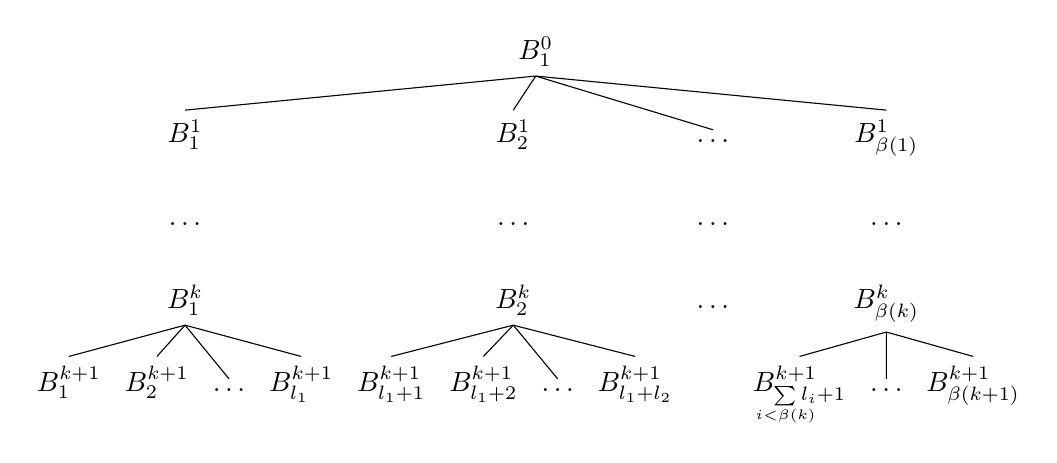
\begin{tikzpicture}
\Tree [. $B^0_1$ [. $B^1_1$ \edge [draw=none]; [. $\ldots$ \edge [draw=none]; [. $B^k_1$ [. $B^{k+1}_1$ ] [. $B^{k+1}_2$ ]  [. $\ldots$ ] [. $B^{k+1}_{l_1}$ ] ] ] ] 
[. $B^1_2$ \edge [draw=none]; [. $\ldots$ \edge [draw=none]; [. $B^k_2$ [. $B^{k+1}_{l_1 + 1}$ ] [. $B^{k+1}_{l_1 + 2}$ ] [. $\ldots$ ] [. $B^{k+1}_{l_1 + l_2}$ ] ] ] ] 
[. $\ldots$  \edge [draw=none]; [. $\ldots$ \edge [draw=none]; [. $\ldots$ ] ] ]
[.$B^1_{\beta(1)}$ \edge [draw=none]; [. $\ldots$ \edge [draw=none]; [.$B^k_{\beta(k)}$ [. $B^{k+1}_{\sum\limits_{\mathclap{i < \beta(k)}}  l_i + 1 }$ ] [. $\ldots$ ] [. $B^{k+1}_{\beta(k+1)}$ ] ] ] ] ]
\end{tikzpicture}
\end{center}
\end{frame}

\begin{frame}{Recursive $\rho$-orderings}
	
%Note to self: write notation on the board, $\Gamma_S$ and $\beta(k)$

	\begin{itemize}
		\item $\rho_{k+1}-$ordering of $S_{\gamma_{k+1}}$ is found by selecting elements of each $B^k_i$ in order as much as possible, and skipping to $B^k_{i+1}$, when it is not possible.
		\pause
		\item  to build a $\rho-$ordering of $S$ from the above, it suffices only to make a choice of centres for each of $B^k_i$'s.
	\end{itemize}
%Note to self: talk about shuffles
\end{frame}


\begin{frame}{Semi-regularity}
%Note to self: define semi-regularity	
\begin{proposition}
	If $S$ is a semi-regular ultrametric space, $\delta$ is the characteristic sequence of $S$, $\beta$ is the structure sequence of $S$, and $\alpha$ is the sequence describing the semi-regularity, then
	\[v_{\gamma_k}(\delta(n)) =  \lfloor\frac{n}{\beta(k)}\rfloor - \lfloor\frac{n}{\beta(k+1)}\rfloor = \sum_{j=1}^{\alpha(k)-1} \lfloor \frac{n + j\cdot \beta(k)}{\alpha(k)\beta(k)} \rfloor\]
\end{proposition}

\end{frame}


\begin{frame}{Regularity}
	%Note to self: define regularity
\begin{proposition}
	Let $S$ be a regular, tame subset of a compact ultrametric space with $\gamma_k = q^{c_k}$ for some $c_k \in \mathbb{Q}$ and for all $k \in \mathbb{N} \cup 0$. Then 
	\[v_{q}(\delta(n)) =  c_0n + \sum_{k=1}^{\infty} (c_{k} - c_{k-1}) \cdot \lfloor\frac{n}{q^{k}}\rfloor \]
	and 
	\[log_q(\omega(S)) = \lim_{n\to\infty} c_0 + \frac{1}{n}\sum_{k=1}^{\infty} (c_{k} - c_{k-1}) \cdot \lfloor\frac{n}{q^{k}}\rfloor  \]
\end{proposition}
\end{frame}

\begin{frame}
	\begin{itemize}
		\item  Semi-regularity implies the presence of a ``well-balanced" partition of $S$.
		\pause
		\item Regularity shows us that we can recover a notion of scaling, when the conditions are right.
		\pause 
		\item Taken together, they extend the toolkit for computing capacity without appealing to algebraic structure\only<+>{.}\only<+->{!} 
	\end{itemize}
\end{frame}


\begin{frame}{Product Space}
\begin{proposition}
	Let $(M_i, \rho_i)$, for $i$ in some finite index set $I$, be a collection of metric spaces and suppose $\rho_i$ is an ultrametric for each $i$. Then $(M,\rho_\infty)$ is an ultrametric space, where $M=M_1 \times M_2 \times \ldots \times M_n$ and $\rho_\infty$ is the metric described above.
\end{proposition}
\pause
\begin{itemize}
	\item Let $M=(\mathbb{Z}^n, \rho_{p, \infty})$ be the ultrametric space with points equal to the $n$-fold product of $(\mathbb{Z}, \rho_p)$ (for $n < \infty$) for some fixed prime $p$. The valuative capacity of $M$ is  $(\frac{1}{p})^{\frac{1}{p^n-1}}$.
	\pause
	\item What about primes $p \neq q$?
\end{itemize}
\end{frame}

\begin{frame}{Product Space: primes $p \neq q$}
	\begin{itemize}
		\item These spaces do not have a scaling property and they are not regular.
		\pause
		\item We use the fact that they are semi-regular and study the exponent of each prime in turn.
	\end{itemize}
\end{frame}

\begin{frame}{Product Space: $(\mathbb{Z},\rho_2) \times (\mathbb{Z},\rho_3)$}
\begin{lemma}
	Let $S = (\mathbb{Z},\rho_2) \times (\mathbb{Z},\rho_3) $ and consider the $k^{th}$ element of the $\beta$ sequence of $S$, $\beta(k) = 2^i \cdot 3^j$. If $k$ is such that $\gamma_k=2^{-i}$ for some $i$, then $j$ counts the numbers $a \in \mathbb{Z}_{\geq 0}$ such that $3^a < 2^{i}$.
\end{lemma}
\pause
\begin{proof}
	\begin{itemize}
	\item $\Gamma_S$ is strictly monotone decreasing and each $\gamma_k$ is equal to a non-positive power of $2$ or $3$. \pause
	\item If $\gamma_k = 2^i$, then all non-positive powers of $3$ and $2$ which are greater than $2^i$ must be equal to some $\gamma_j$, $0 \leq j < k$.\pause %That is, $2^i$ only appears in the $\Gamma_S$ sequence after all larger powers of $2$ and $3$ have been exhausted.
	\item Since we are only considering the case $\gamma_k$ is a power of $2$, this includes all of the smaller powers of $3$.
	\end{itemize}
\end{proof}
\end{frame}
\begin{frame}{Product Space: $(\mathbb{Z},\rho_2) \times (\mathbb{Z},\rho_3)$}
	 \[v_{\gamma_{\frac{1}{2}}}(\delta(n)) = \sum_{i=1}^\infty i \cdot \lfloor\frac{n + 2^i \cdot 3^{\lceil \frac{i}{log_2(3)}\rceil}}{2^{i+1}\cdot 3^{\lceil \frac{i}{log_2(3)}\rceil}} \rfloor\]
		\pause
	 \[v_{\gamma_{\frac{1}{3}}}(\delta(n)) = \sum_{i=1}^\infty i \cdot (\lfloor\frac{n + 2^{\lceil \frac{i}{log_3(2)}\rceil} \cdot 3^i}{2^{\lceil \frac{i}{log_3(2)}\rceil}\cdot 3^{i+1}} \rfloor + \lfloor\frac{n + 2^{\lceil \frac{i}{log_3(2)}\rceil+1} \cdot 3^i}{2^{\lceil \frac{i}{log_3(2)}\rceil}\cdot 3^{i+1}} \rfloor) \]
\end{frame}

\begin{frame}{Product Space: primes $p \neq q$}
\begin{conjecture} Finite products of $(\mathbb{Z}, \rho_{p_i})$ for distinct primes, $p_i$, have transcendental valuative capacity.\\ \end{conjecture}
\end{frame}


\begin{frame}
\frametitle{references}
\begin{thebibliography}{9}
%	\bibitem[Ac]{na} N.L. Ackerman, Completeness in Generalized Ultrametric Spaces, \textit{$p$-Adic Numbers, Ultrametric Analysis, and Applications} \textbf{5(2)} (2013), 89-105.
%	\bibitem[Am]{amice} Y. Amice, Interpolation $p$-adique, \textit{Bull. Soc. Math. France} \textbf{92} (1964) 117-180.
%	\bibitem[BR]{rum} M. Baker and R Rumely, \textit{Potential Theory and Dynamics on the Berkovich
%		Projective Line}, Amer. Math. Soc., Providence, 2010.
	\bibitem[B1]{mb2} M. Bhargava, $P$-orderings and polynomial functions on arbitrary subsets of Dedekind
	rings, \textit{J. reine angew. Math.}, \textbf{490} (1997), 101-127.
	\bibitem[B2]{mb1} M. Bhargava, The factorial function and generalizations, \textit{Am. Math. Monthly}
	\textbf{107} (2000), 783-799.
%	\bibitem[B3]{mb3} M. Bhargava, On $P$-orderings, Rings of Integer Valued Polynomials and Ultrametric
%	Analysis, \textit{Journal of the Amer. Math. Soc.} \textbf{22(4)} (2009), 963-993.
%	\bibitem[Ca]{dgc}  D. Cantor, On an extension of the definition of transfinite diameter and some applications, \textit{J. reine angew. Math} \textbf{316} (1980), 160-207.  
	\bibitem[Ch]{jlc} J.-L. Chabert, Generalized factorial ideals, \textit{Commutative algebra, Arab. J. Sci. Eng.
		Sect. C} \textbf{26} (2001), 51-68.
%	\bibitem[CEF]{cef} J.-L.Chabert, S. Evrard, Y. Fares, Regular subsets of valued fields and Bhargava’s $v$-orderings, \textit{Math. Z.} \textbf{274} (2013) 263-290.
%	\bibitem[EF]{ef} S. Evrard and Y. Fares, $p$-adic subsets whose factorials satisfy a generalized Legendre
%	formula, \textit{London Math. Soc.}, \textbf{40} (2008), 37-50.
%	\bibitem[FP]{fp} Y. Fares, S. Petite, The valuative capacity of subshifts of finite type, \textit{J. Number Theory} \textbf{158}
%	(2016), 165-184.
	%\bibitem[GV]{gvdp} Lothar Gerritzen and Marius van der Put, Schottky Groups and Mumford Curves.
	\bibitem[F]{fek} M. Fekete, Uber die Verteilung der Wurzelen bei gewisser algebraiche Gleichun-
	gen mit ganzzahligen Koeffizienten, \textit{Math. Zeits.} \textbf{17} (1923), 228-249.
	\bibitem[J1]{kj} K. Johnson, $p$-orderings, Fekete $n-$tuples and capacity in ultrametric spaces (in preparation).
%	\bibitem[J2]{kj2} K. Johnson, Limits of characteristic sequences of integer-valued polynomials on
%	homogeneous sets, \textit{J. Number Theory} \textbf{129} (2009), 2933-2942.
%	\bibitem[M]{mun} J. Munkres, \textit{Topology}, Prentice Hall Inc., Upper Saddle River NJ, 2000.
%	\bibitem[Ra1]{rand} T. Ransford, \textit{Potential Theory in the Complex Plane}, Cambridge University Press, Cambridge, 1995.
%	\bibitem[Ra2]{rand2} T. Randsford, Computation of Logarithmic Capacity, \textit{Comp. Methods Function Theory} \textbf{10} (2010), 555-578.
%	\bibitem[Ro]{ar} A.M. Robert, \textit{A course in p-adic analysis}, Springer-Verlag, New York, 2000.
%	\bibitem[S]{sim} B. Simon, Equilibrium measures and capacities in spectral theory, \textit{Inverse Probl. Imaging} \textbf{1}:4 (2007), 713–772. 
%	\bibitem[W]{wer} J. Wermer, \textit{Potential Theory}, Springer Lecture Notes in Mathematics, \textbf{408}, Providence, 1981.
\end{thebibliography}\end{frame}

\end{document}

%\appendix
%\section*{Maple Code}

In this appendix, we include for reference the Maple code that was used to investigate the capacity of product spaces. The result of this investigation also influenced the development of Chapters 3 and 4. There are three procedures listed here.

\begin{enumerate}
	\item The first procedure, \texttt{ComputePadicProductOrdering}, takes as input a list indicating a finite set of primes, $p_1, 
\ldots, p_n$, and an integer $m$ and returns the first $m$ terms of a $\rho_\infty-$ordering of $(\mathbb{Z}_{p_1} \times \ldots \times \mathbb{Z}_{p_1} )$. This is done explicitly by following the algorithm described in Chapter 3.
	\item The next procedure, \texttt{ComputePartialRhoSeq}, computes the resulting $\rho_\infty-$sequence for a product space by multiplying out the distances given by a $\rho_\infty-$ordering. It takes as input a metric and a matrix representing a $\rho_\infty-$ordering for a product space and returns a number indicating the value of the $n^{th}$ characteristic sequence, where $n$ is the row dimension of the input matrix. These two procedures therefore result in the naive computation of the partial characteristic sequence of a product space, found by explicitly calculating a $\rho_\infty-$ordering and the $\rho_\infty-$sequence in turn.
	
	\item The final procedure, \texttt{FastPartialRhoSeq}, exploits the fact that the terms occurring in the characteristic sequence of a product space are all powers of the primes specifying the space. It takes as input the (beginning of) the sequence of decreasing distances and a list of primes, specifying the space. If $k$ distances are specified in $A$, it returns the $\beta(k)^{th}$ term in the characteristic sequence, where $\beta$ is the structure sequence.
\end{enumerate}

\newpage
\lstinputlisting{code/Padic_Product_Ordering.txt}


\newpage
\lstinputlisting{code/Partial_Rho_Sequence.txt}

\newpage
\lstinputlisting{code/Fast_Partial_Rho_Sequence.txt}
	

\begin{thebibliography}{9}
\bibitem[Ac]{na} Nate Ackerman,  Completeness in Generalized Ultrametric Spaces
\bibitem[Am]{amice} Amice. Interpolation p-adique, Bull. Soc. Math. France 92 (1964) 117–180.
\bibitem[BR]{rum} Matthew Baker and Robert Rumely. Potential theory and dynamics on the Berkovich Projective Line.
\bibitem[B1]{mb1} Manjul Bhargava. The factorial function and generlizations
\bibitem[B2]{mb2} Manjul Bhargava. $P$-orderings and polynomial functions on arbitrary subsets of Dedekind rings.
\bibitem[B3]{mb3} Manjul Bhargava. On $ P$-orderings, rings of integer-valued polynomials, and ultrametric analysis
\bibitem[Ca]{dgc}  D.G. Cantor. On an extension of the definition of transfinite diameter and some applications.  
\bibitem[Ch]{jlc} Jean-Luc Chabert. Generalized Factorial Ideals.
\bibitem[CEF]{cef} Jean-Luc Chabert, Sabine Evrard and Youssef Fares. Regular subsets of valued fields and Bhargava’s $v$-orderings
\bibitem[EF]{ef} Sabine Evrard and Youssef Fares. $p$-adic subsets whose factorials satisfy a genearlized Legendre formula.
\bibitem[FP]{fp} Youssef Fares and Samuel Petite. The valuative capcity of subshifts of finite type.
\bibitem[GV]{gvdp} Lothar Gerritzen and Marius van der Put, Schottky Groups and Mumford Curves.
\bibitem[F]{fek} Fekete.
\bibitem[J1]{kj} Keith Johnson, P-orderings and Fekete sets
\bibitem[J2]{kj2} Keith Johnson, that paper that's at school
\bibitem[Ra1]{rand} Thomas Randsford. Potential theory in the complex plane.
\bibitem[Ra2]{rand2} Thomas Randsford. Computation of Logarithmic Capacity.
\bibitem[Ro]{ar} Alain M. Robert. A course in p-adic analysis.
\bibitem[S]{sim} Barry Simon. Equilibrium measures and capacities in spectral theory.
\bibitem[W]{wer} John Wermer. Potential Theory.
\end{thebibliography}
\end{document} 